\chapter{Recurrent neural networks}
\section{Hopfield Network}
A hopfield network is like associative memory where it can reconstruct the input data even if the data is noisy. The network is a chain of neurons where each neuron can take either of one state as +1 or -1. Suppose for a neuron $i$ at given time $t$, the state of the neuron can be expressed as $S_i(t) = +1 $ or $S_i(t) = -1 $. The dynamics of the network evolves in discrete time steps $\Delta$t which means the output of a neuron at time $t$ becomes an input at time $t+1$. Each neuron interacts with each other with a weight matrix $w_{ij}$. The action potential of a neuron $i$ due to the activity of $i-1$ neurons can be given as follows
\begin{equation}
h_i(t) = \sum_{j}w_{ij}S_j(t)
\end{equation}
To demonstrate the working of the hopfield network, we create the network with 3 attractors $T=[1 \ 1;-1 \ -1;1 \ -1]'$ in two different scenarios. One scenarios where we randomly assign the initial states for the network and the other scenario where we assign symmetrical states. The result of these scenarios is shown in the below figure \ref{fig:hop}. In figure \ref{fig:hop1} it can be seen that each initial state reaches a attactor that closer to it. It exhibits a nearest neighbour behaviour. \\
\begin{figure}[!htpb]
	\centering
	\begin{subfigure}[b]{0.5\textwidth}
		\captionsetup{width=0.8\linewidth, format = hang}
		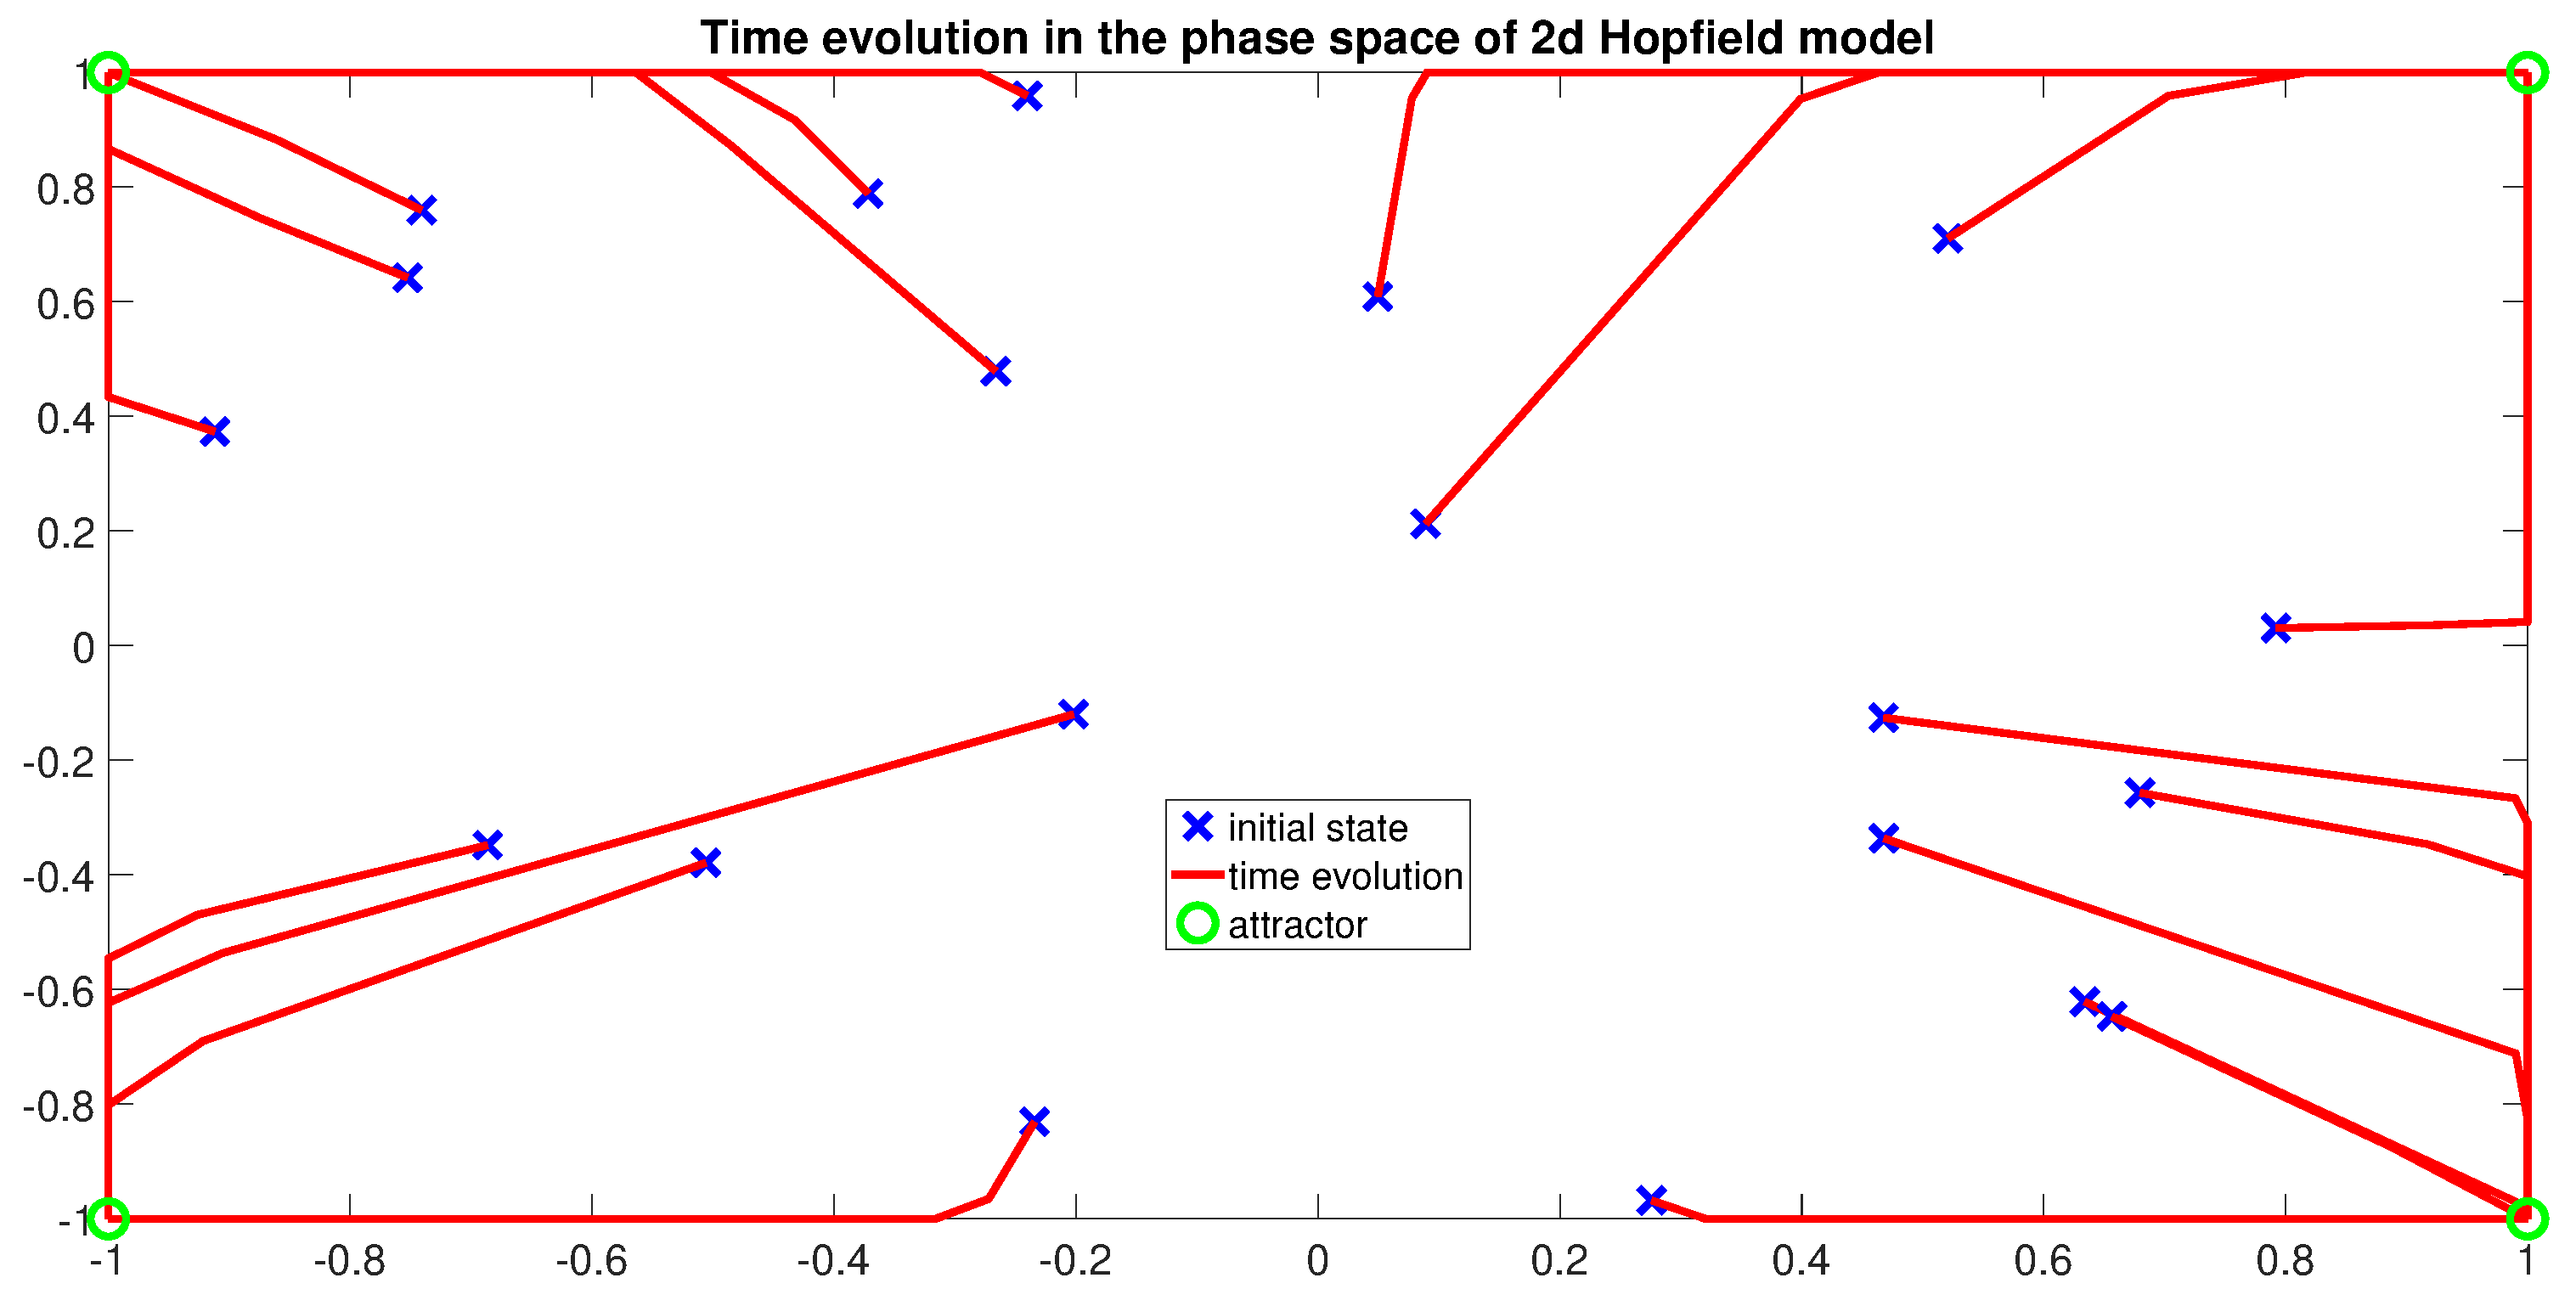
\includegraphics[height = 0.6\textwidth,width = 1\textwidth]{Exercise2/Report/hopfield_1}
		\caption{2 Neuron: Hopfield network with random initial states }\label{fig:hop1}
	\end{subfigure}%
	\begin{subfigure}[b]{0.5\textwidth}
		\captionsetup{width=0.8\linewidth, format = hang}
		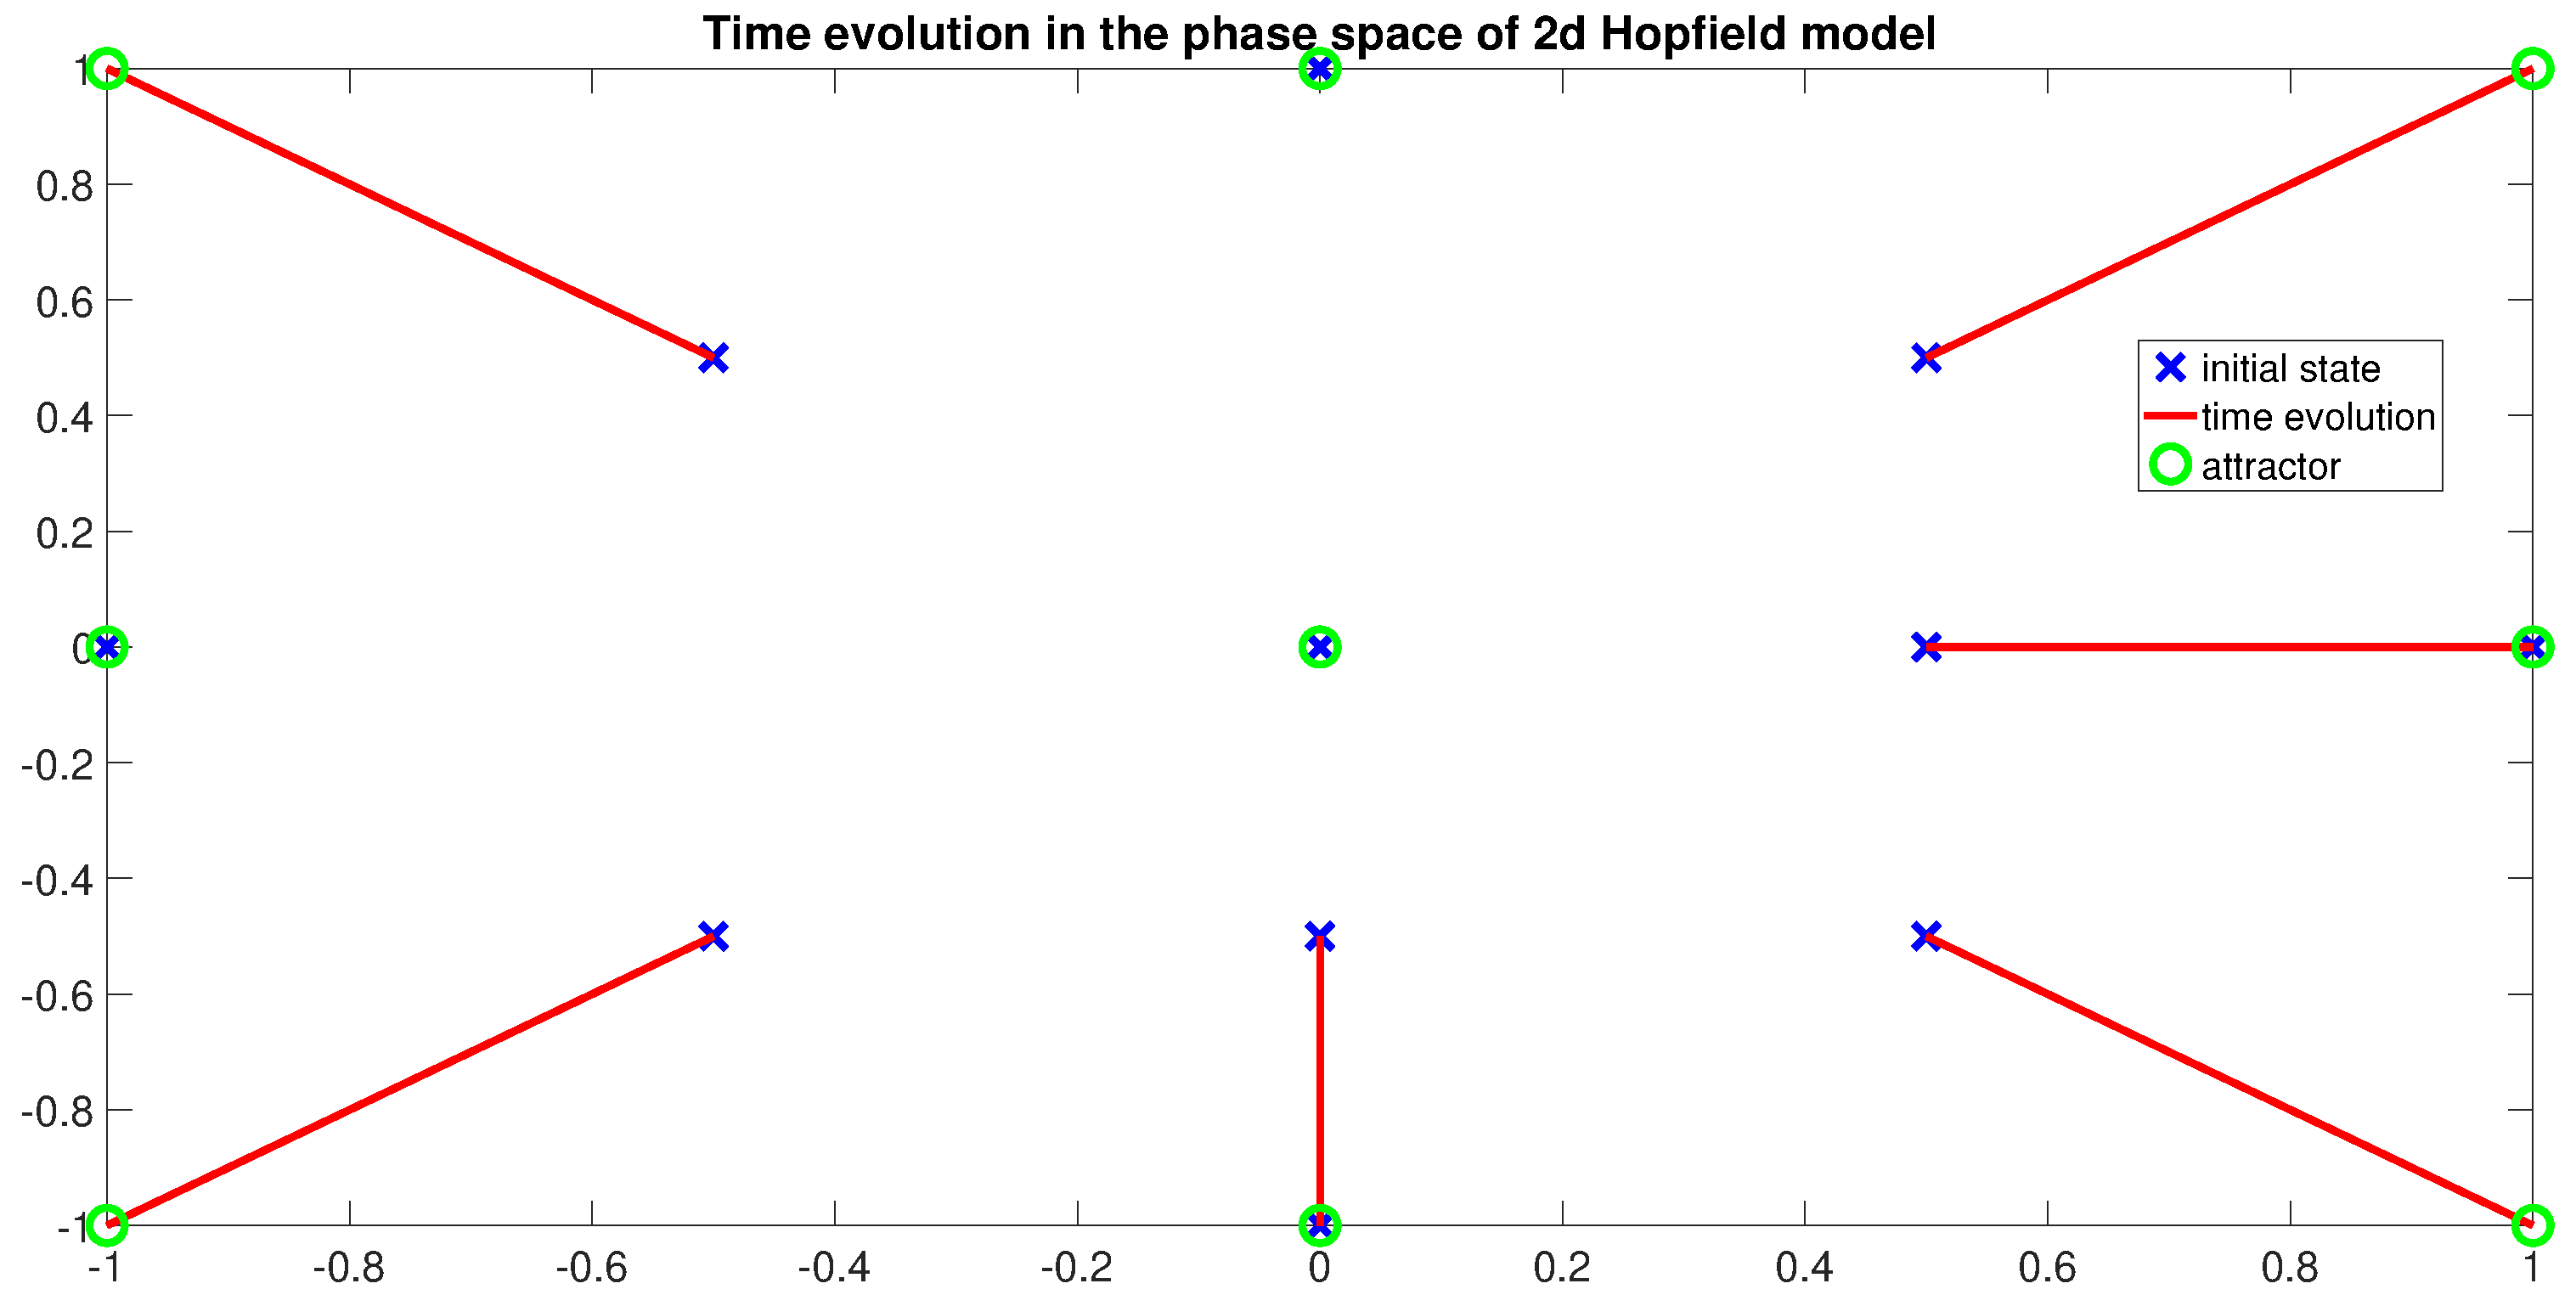
\includegraphics[height = 0.6\textwidth,width = 1\textwidth]{Exercise2/Report/hopfield_3}
		\caption{2 Neuron: Hopfield network with symmetrical initial states}\label{fig:hop3}
	\end{subfigure}%
	\caption{Time evolution in the phase space of 2D Hopfield model }
	\label{fig:hop}
\end{figure}
One thing that can be noticed is that the number of attractors is not the same as how it has been created. The attractors are more in number amd can be seen as green circles in figure \ref{fig:hop}. The networks adds a new attractor at (1,1) known as spurious state in figure \ref{fig:hop1}. Spurious states are a retrieval states that the network uses during the pattern training, which eventually becomes an attractor. The energy in these spurious states is also a local minima. \\

\begin{wrapfigure}{L}{0.4\textwidth}
	\captionsetup{format = hang}
	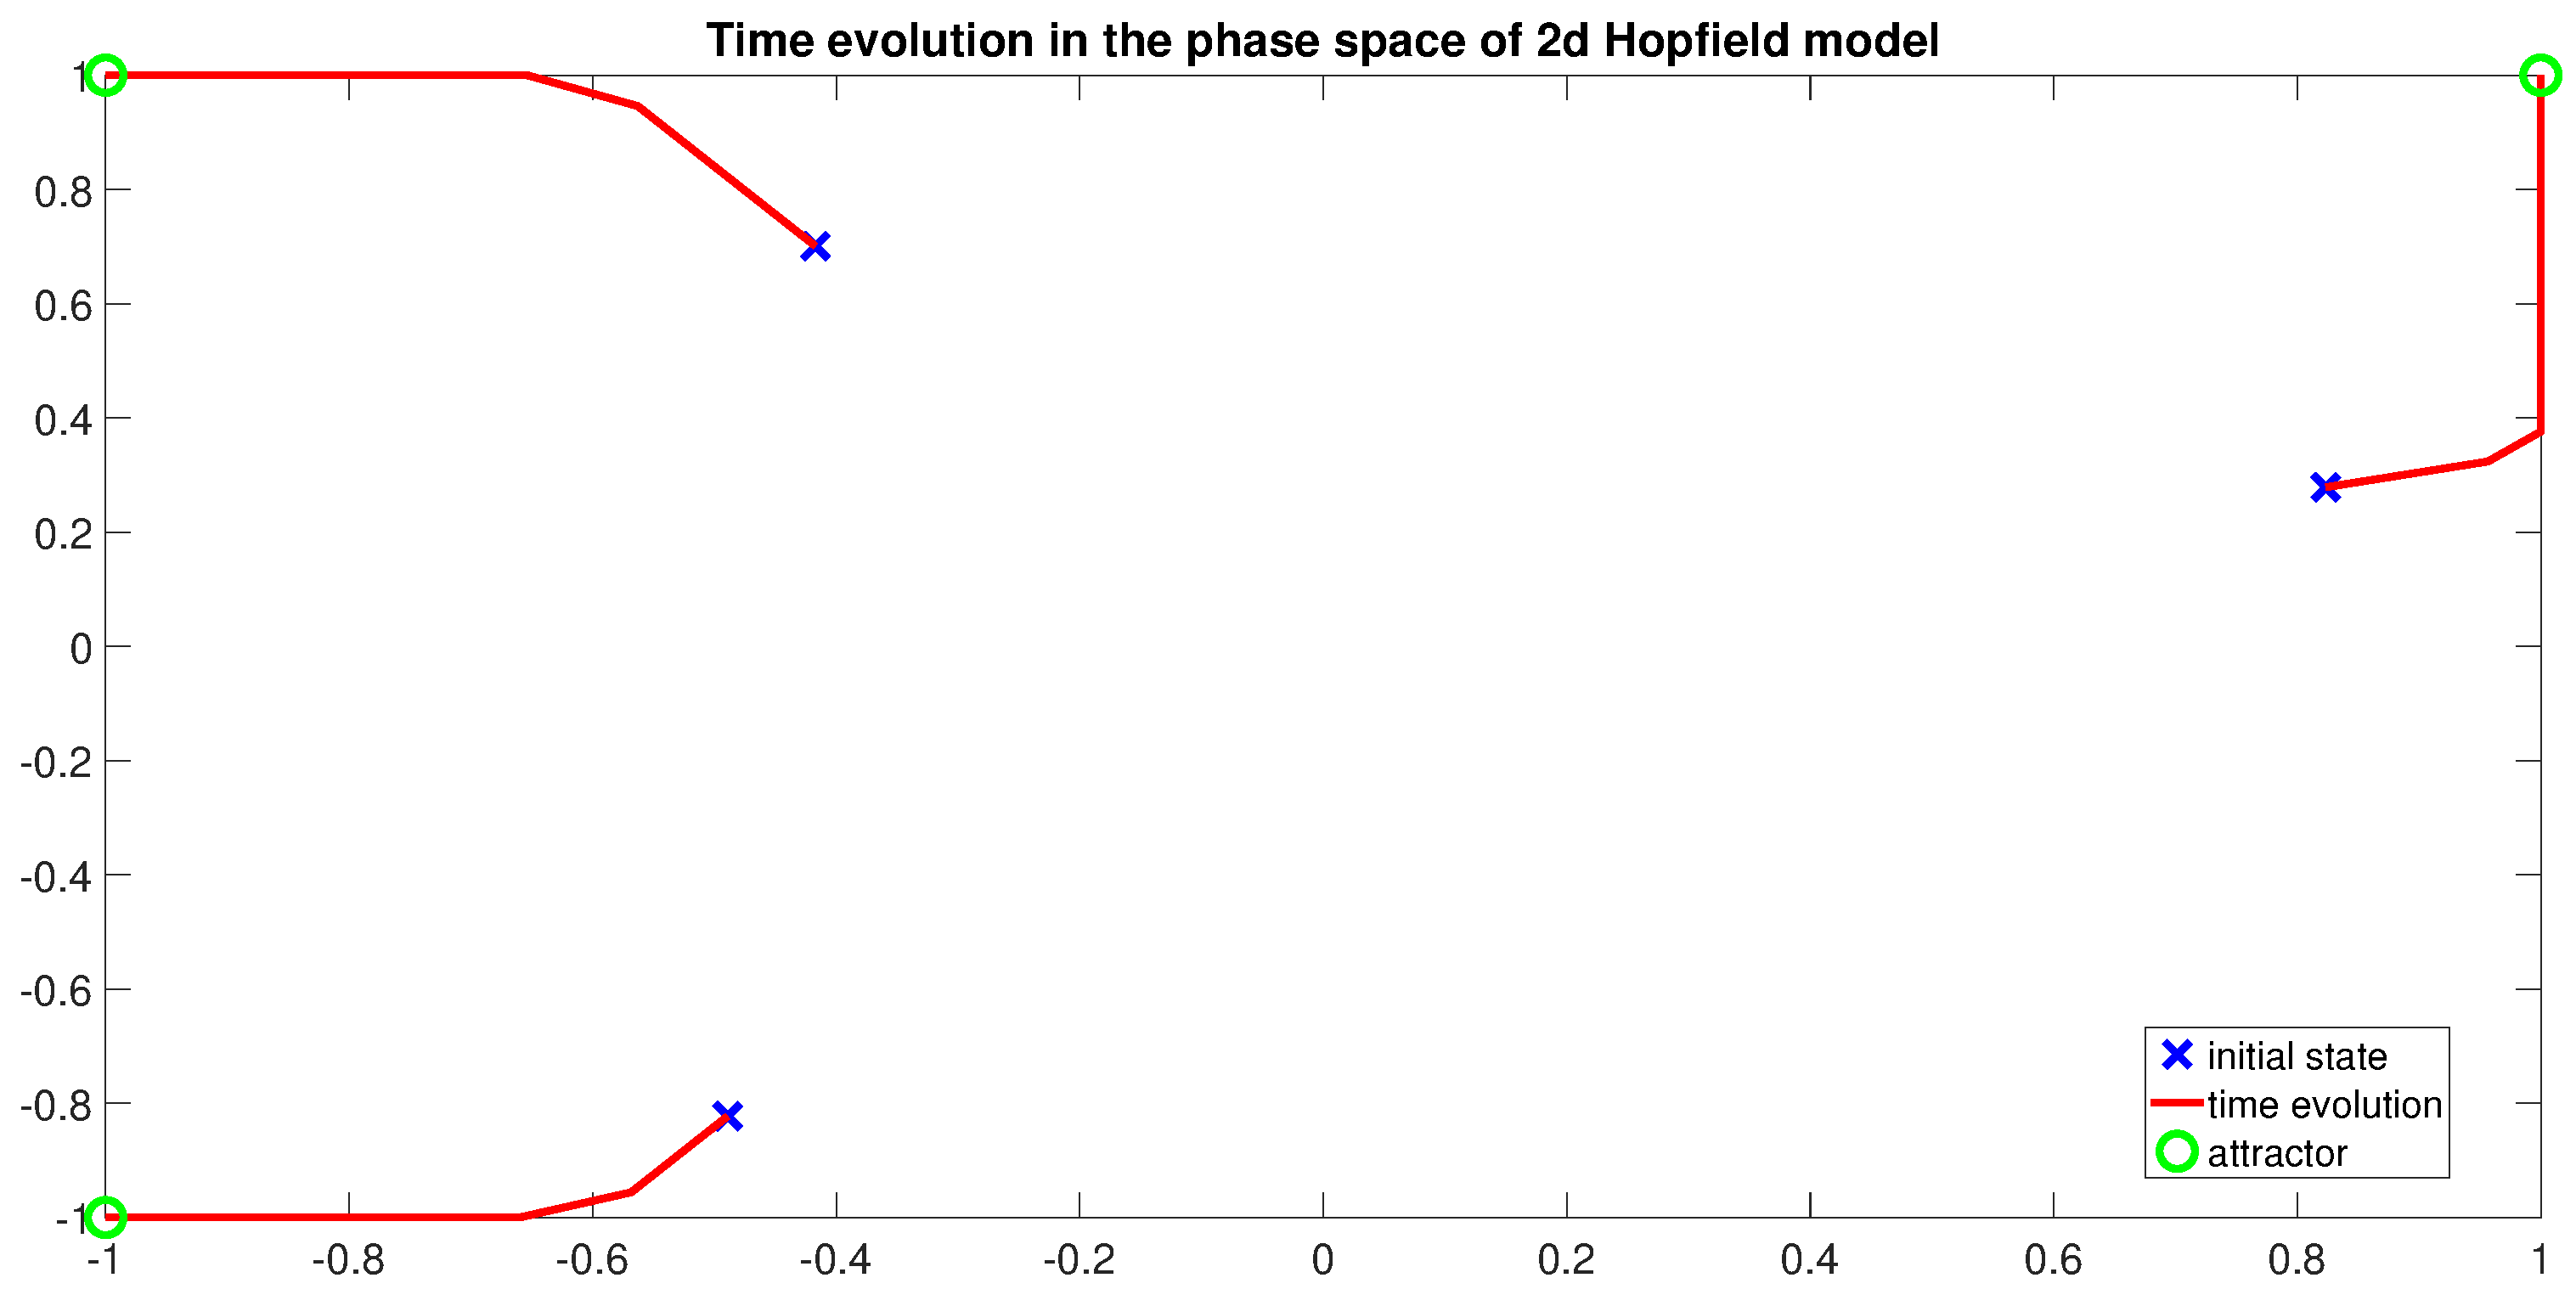
\includegraphics[height = 0.5\textwidth,width = 1\textwidth]{Exercise2/Report/hopfield_2}
	\caption{Hopfield network convergence to an attractor}\label{fig:hop2}
\end{wrapfigure}%
Repeated updates to the network states leads to the convergence to a retrieval state which is a spurious state. In the case of symmetrical states as shown in figure \ref{fig:hop3}, the network adds more spurious states and during convergence some  states become attractors themselves. The number of attractors for symmetrical points are more than random ones. The network takes atleast 15 iterations to converge to an attractor in case of 3 random initial states that is shown in figure \ref{fig:hop2}.\\
In case of a 3 neuron hopfield network, the network correctly converges to the attractors for randomly initialized states as seen in figure \ref{fig:hop3d_1}. But, for symmetrical states, the network produces spurious attractors as seen in figure \ref{fig:hop3d_2}
\begin{figure}[!htpb]
	\centering
	\begin{subfigure}[b]{0.5\textwidth}
		\captionsetup{width=0.8\linewidth, format = hang}
		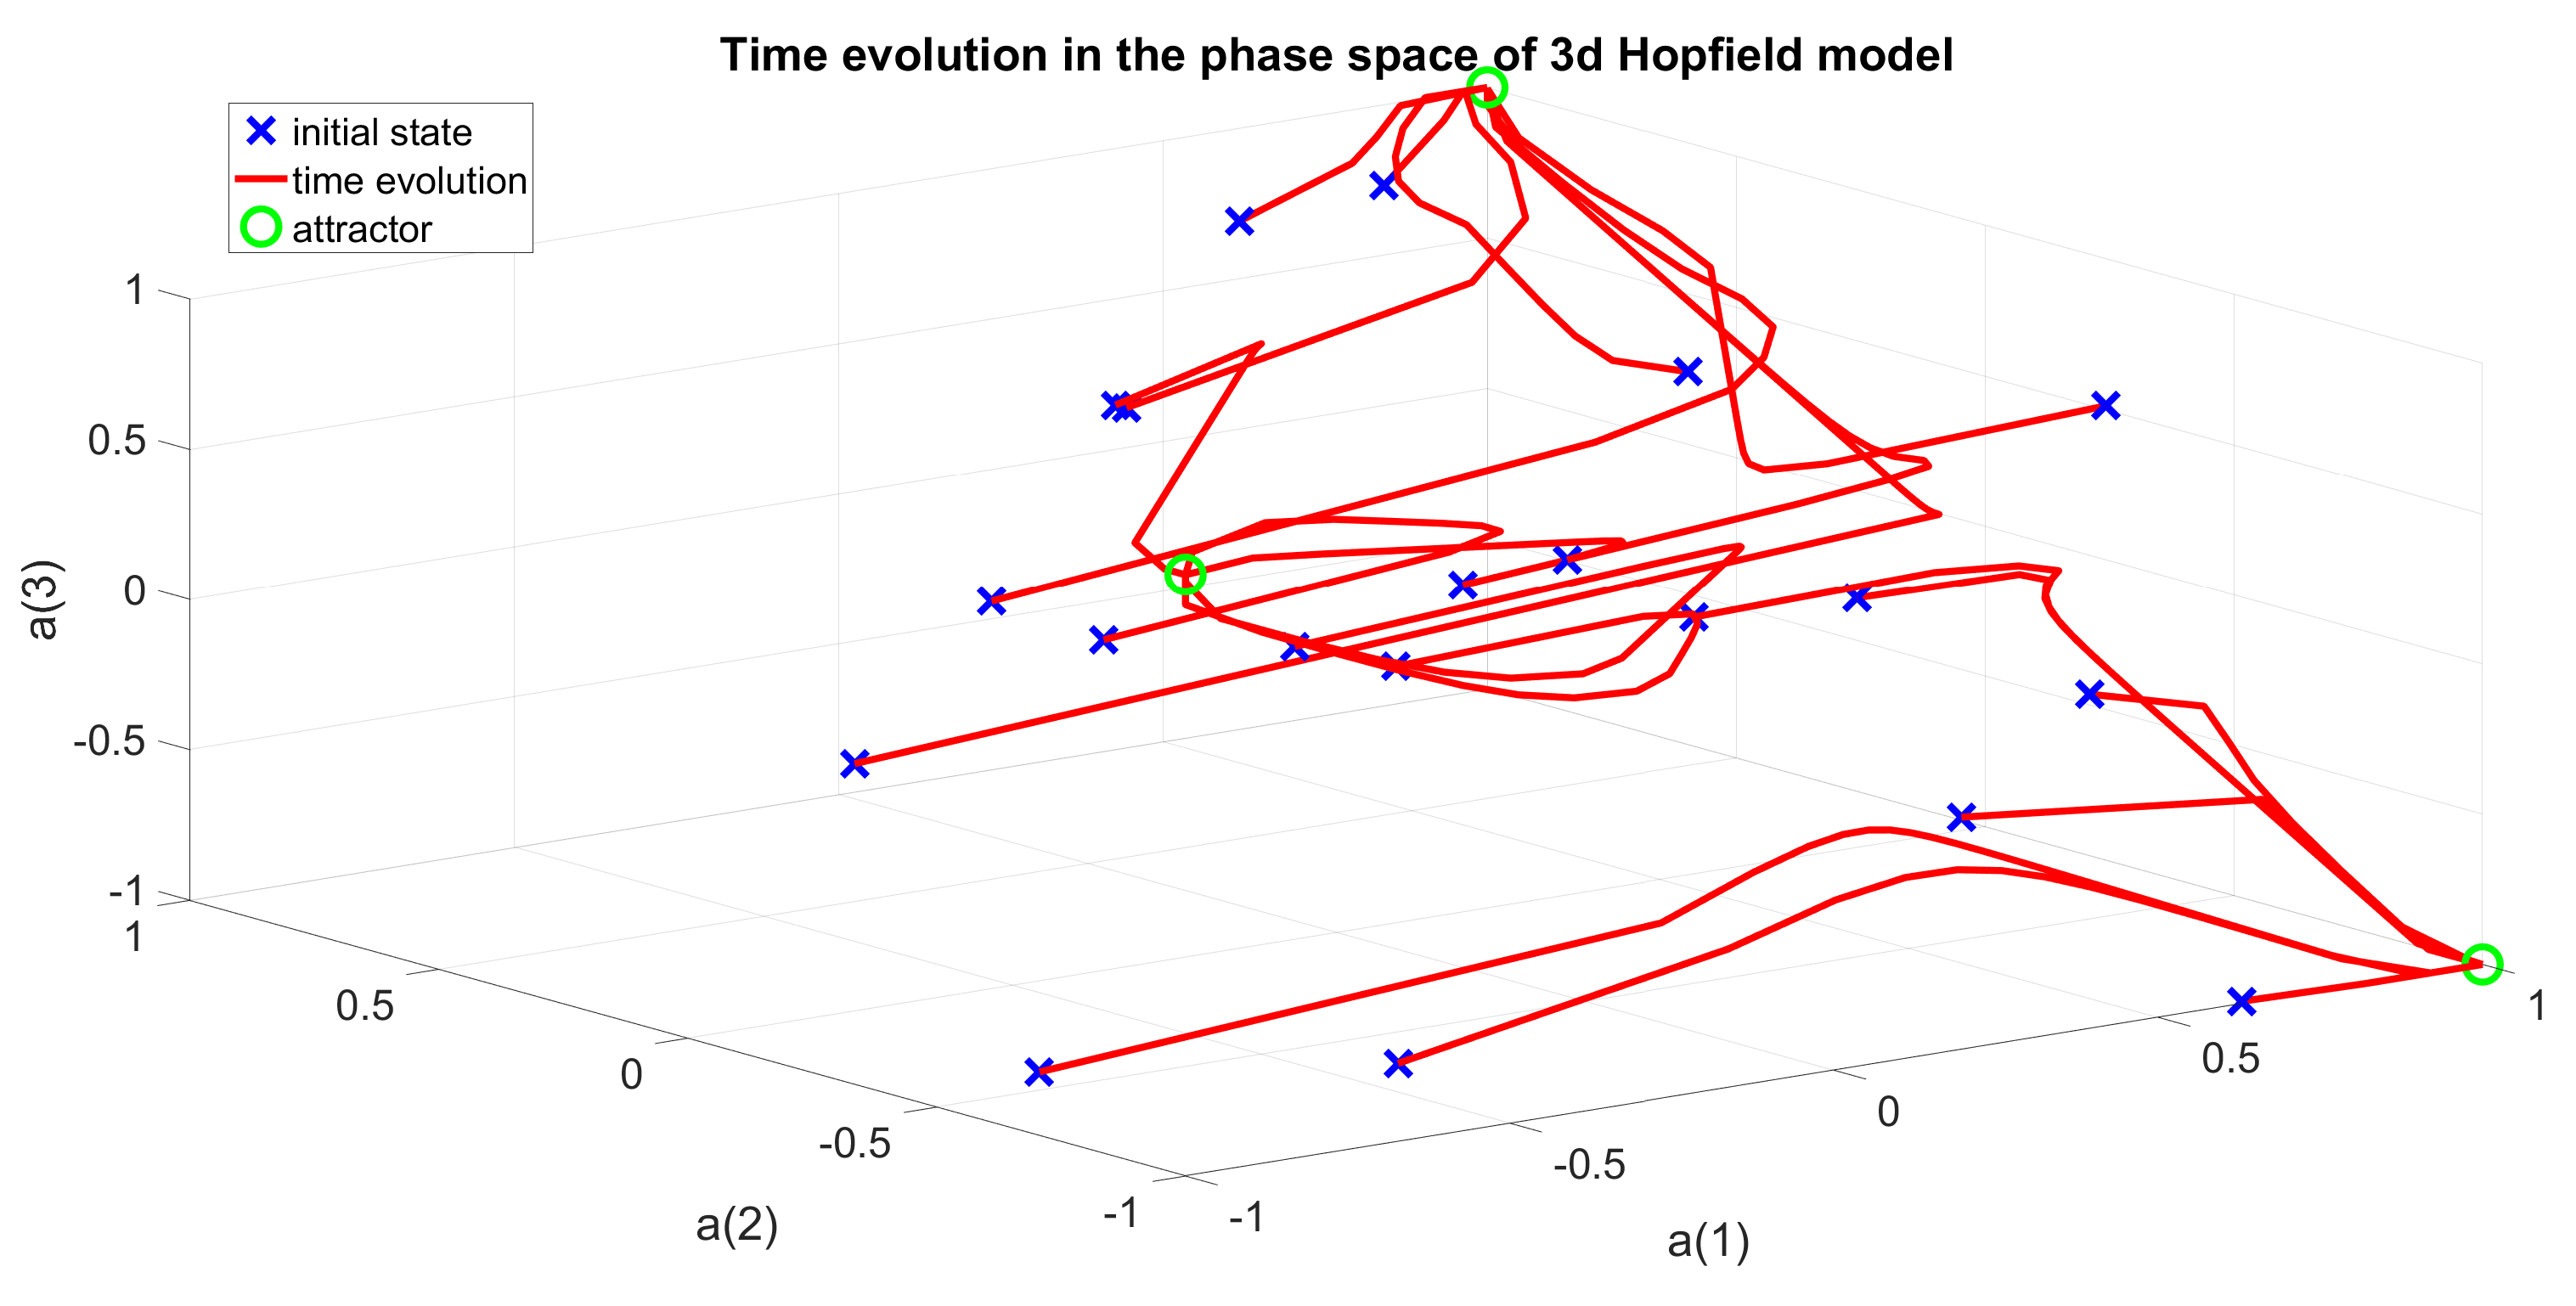
\includegraphics[height = 0.6\textwidth,width = 1\textwidth]{Exercise2/Report/hop3d_1}
		\caption{3 Neuron: Hopfield network with random initial states }\label{fig:hop3d_1}
	\end{subfigure}%
	\begin{subfigure}[b]{0.5\textwidth}
		\captionsetup{width=0.8\linewidth, format = hang}
		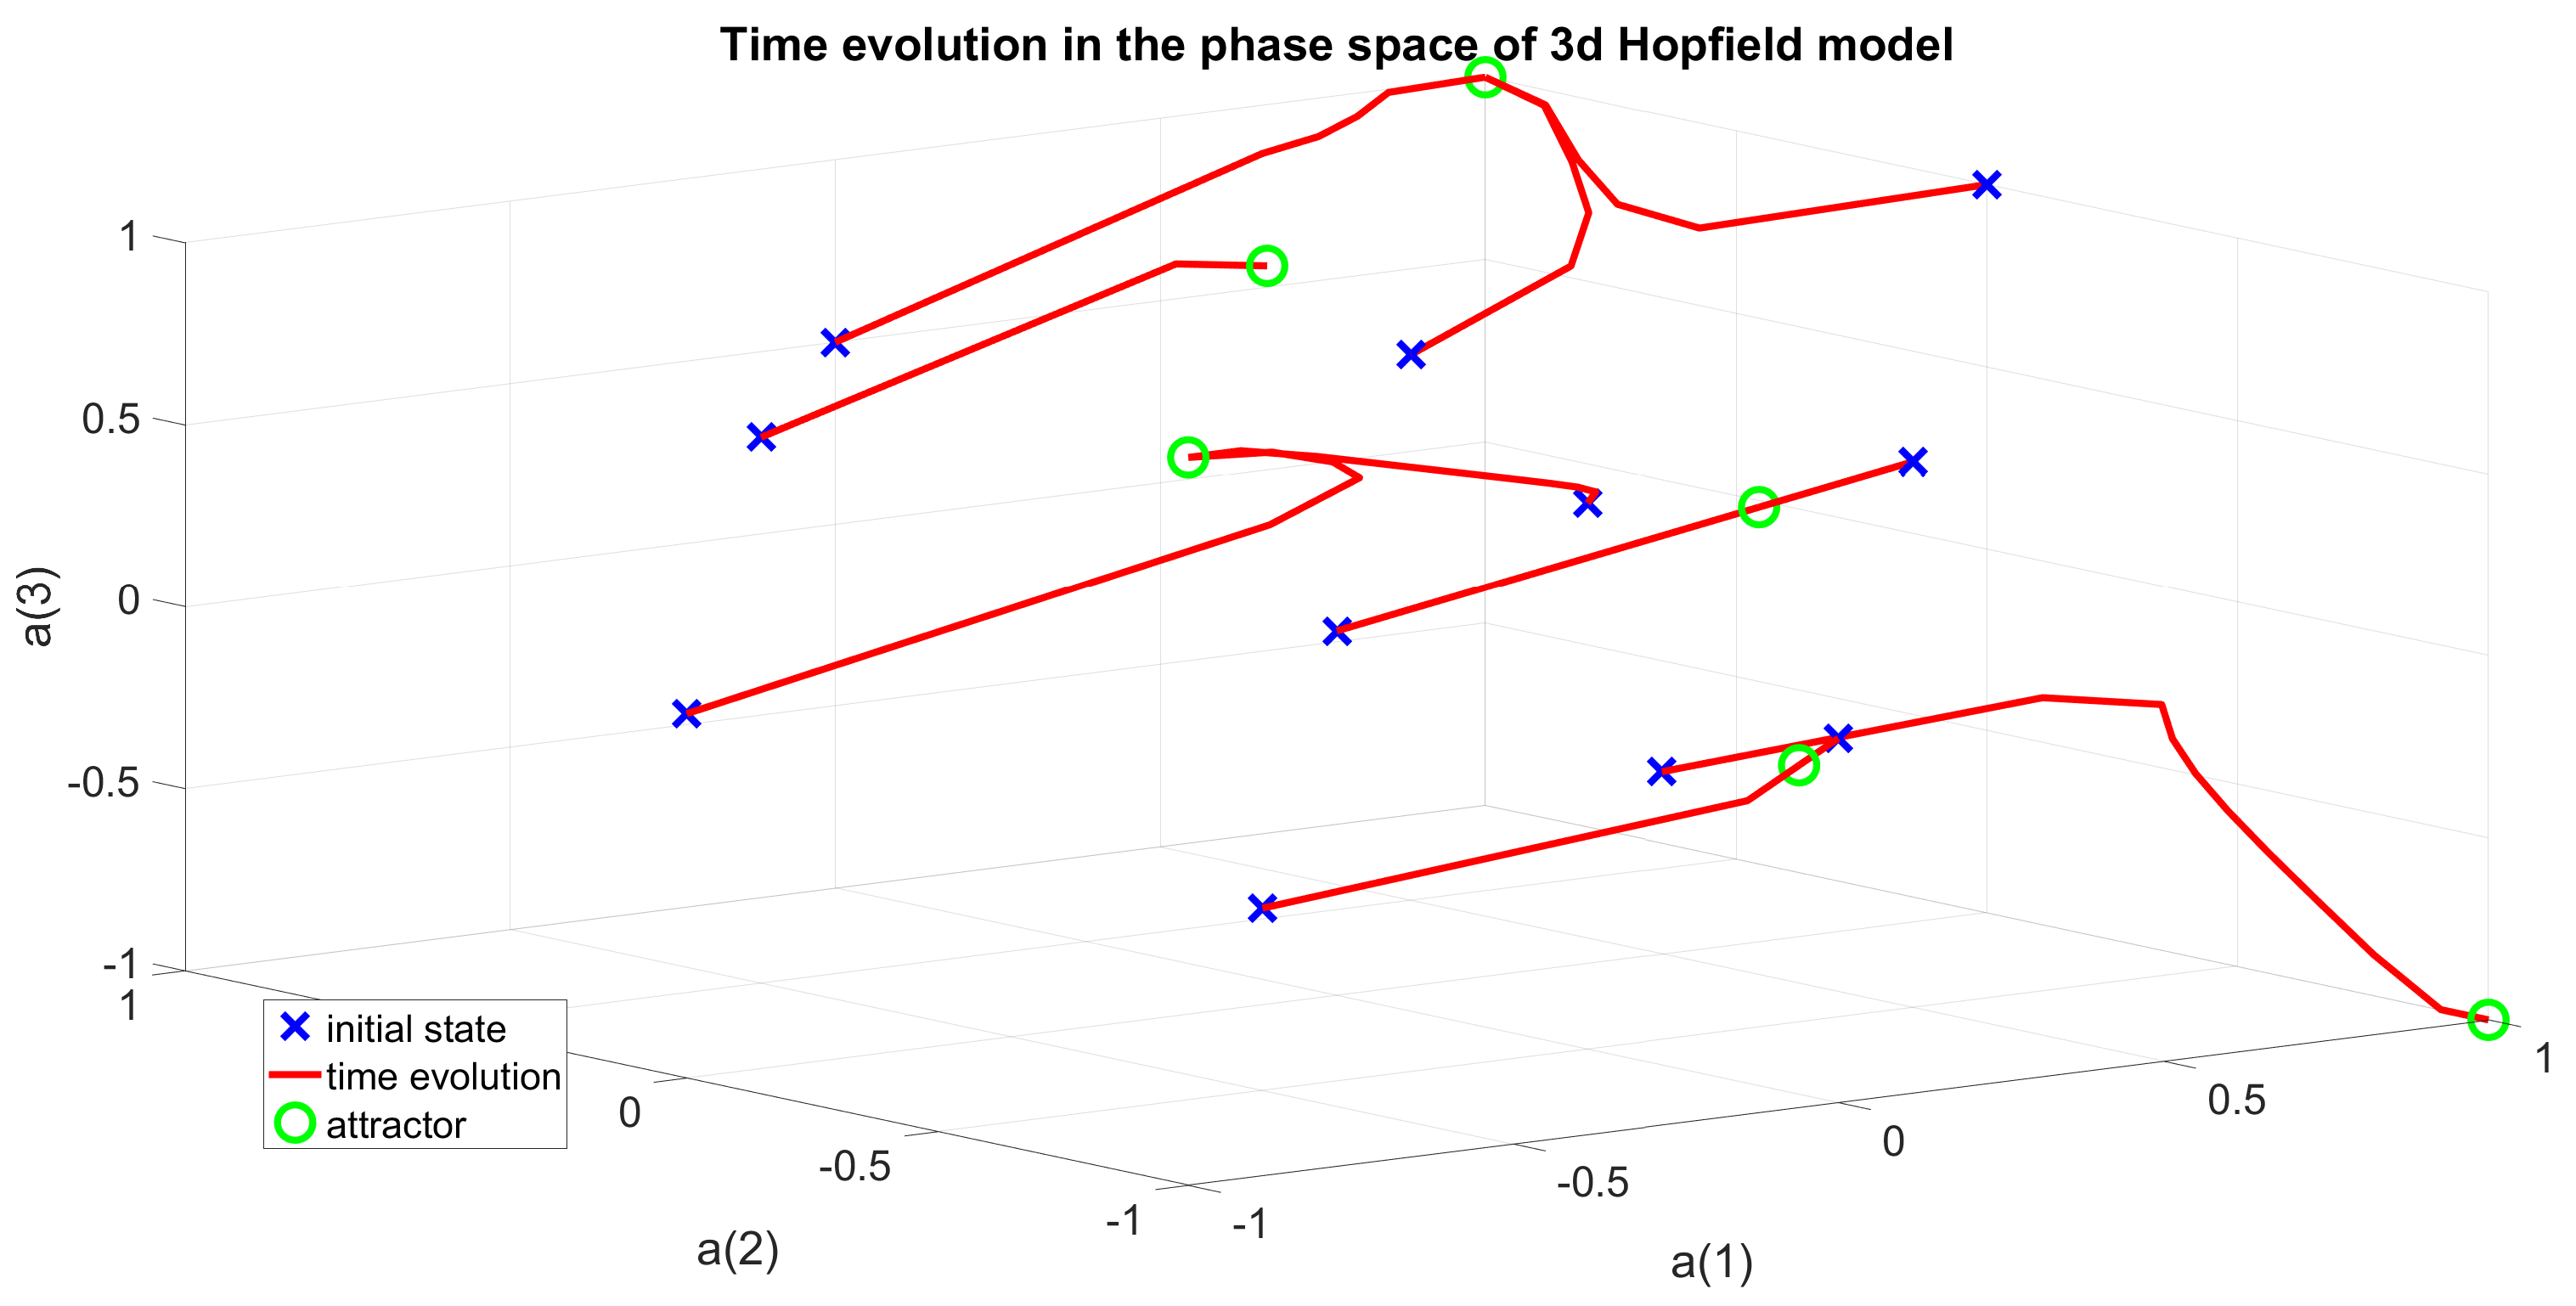
\includegraphics[height = 0.6\textwidth,width = 1\textwidth]{Exercise2/Report/hop3d_2}
		\caption{3 Neuron: Hopfield network with symmetrical initial states}\label{fig:hop3d_2}
	\end{subfigure}%
	\caption{Time evolution in the phase space of 3D Hopfield model }
	\label{fig:hop_3c}
\end{figure}

We then move on to reconstructing the hand written digits using \textit{hopdigit} function. The network is trained with proper handwritten digits which acts as attractors and then inputting different noise levels over the handwritten digits as initial states for reconstruction. The network is tested with four different configurations of noise levels and iterations. The network's behaviour is shown in the figure \ref{fig:hop_digit}. It can be noticed that, for lower levels of noise (say 5) the network is able to reconstruct the pattern correctly to some extent except for one digit. For lighter levels of noise, the networks performance reduces further even after giving higher number of iterations. This could be because the network would have converged to a spurious state which is also a local minima and can be seen in figure \ref{fig:hop_digit3} of digit 2 with Noise level 10 and iterations 50 .\\
\begin{figure}[ht]
	\begin{subfigure}[b]{0.26\textwidth}
		\centering
		\captionsetup{ width=0.8\linewidth, format = hang}
		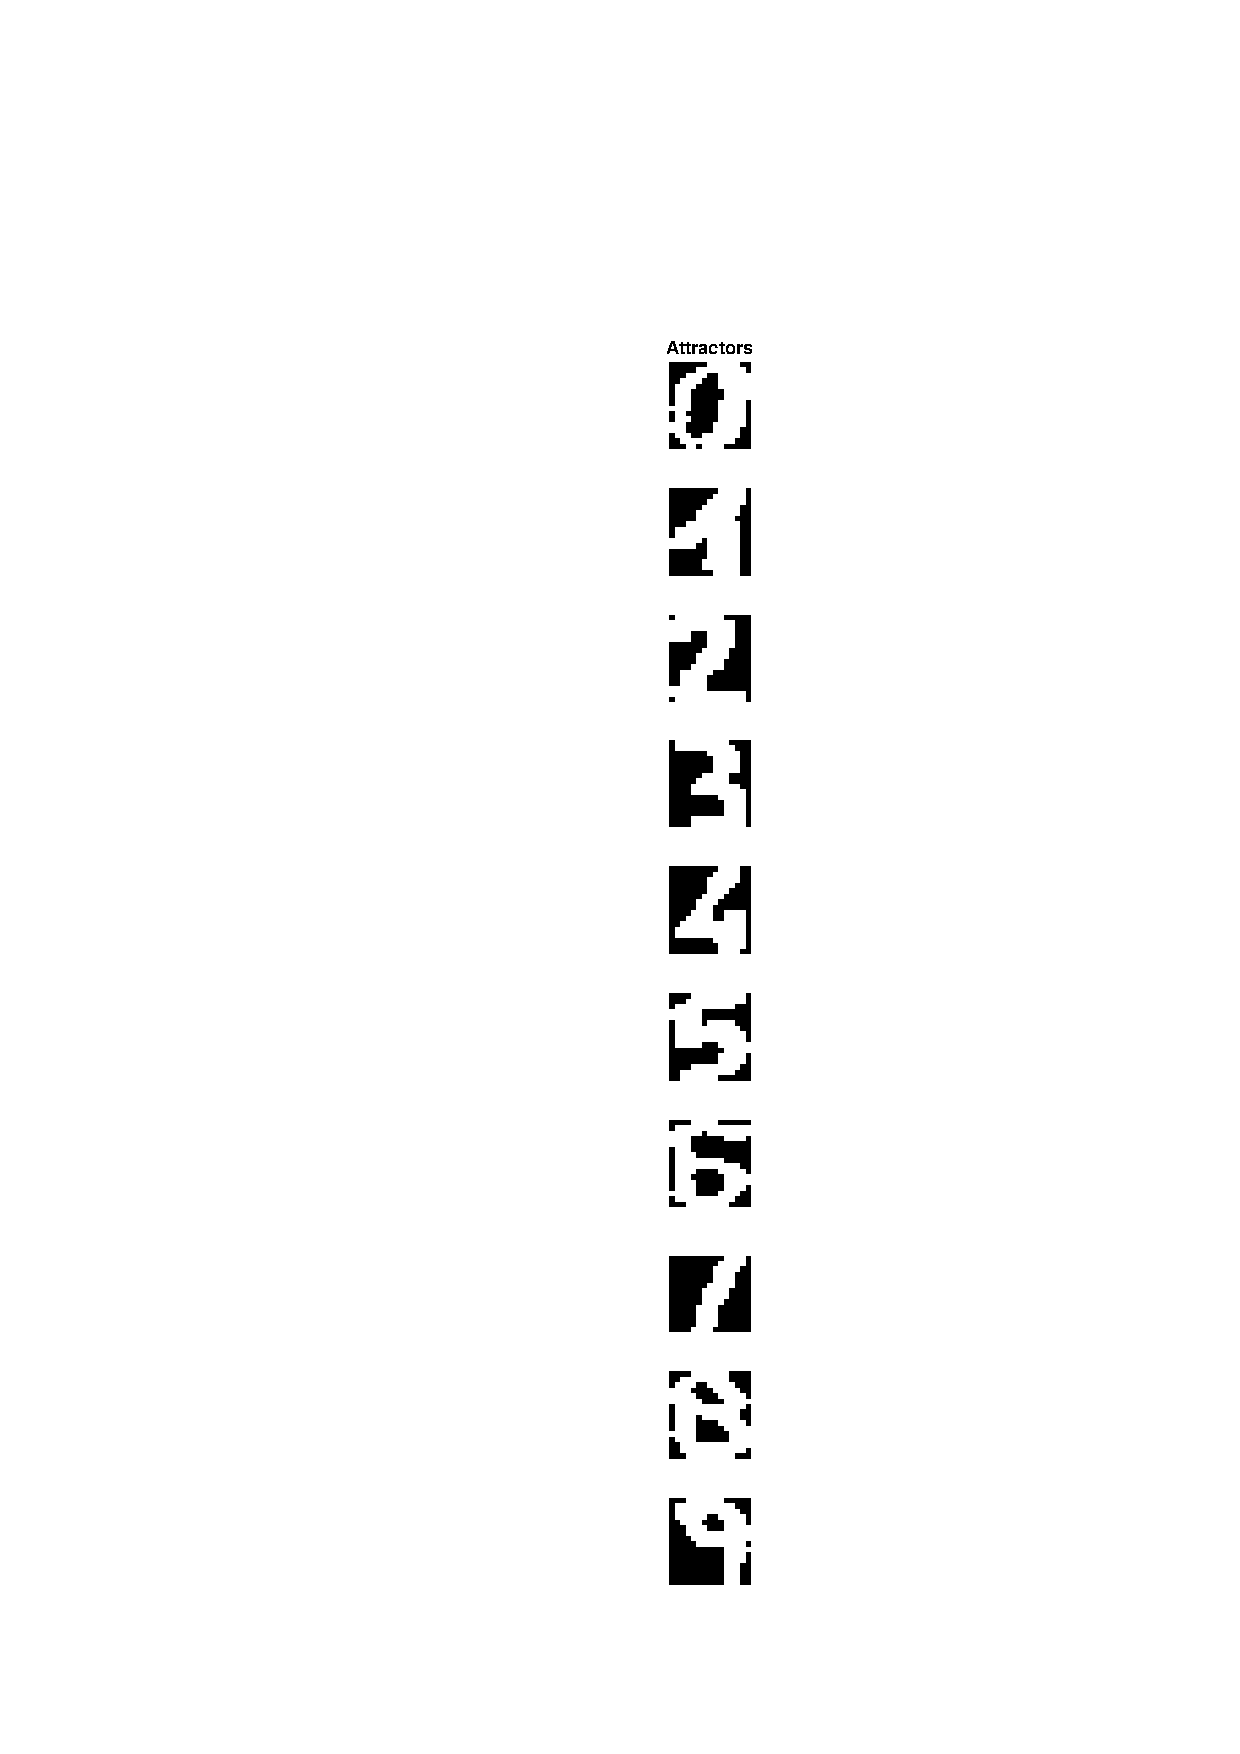
\includegraphics[height = 1.2\textwidth, width = 0.8\textwidth]{Exercise2/Report/hdr_n5_itr10.jpg}
		\caption{Noise Level = 5; Iterations = 10}\label{fig:hop_digit1}
	\end{subfigure}%
	\begin{subfigure}[b]{0.26\textwidth}
		\centering
		\captionsetup{width=0.8\linewidth, format = hang}
		\includegraphics[height = 1.2\textwidth, width = 0.8\textwidth]{Exercise2/Report/hdr_n5_itr80.jpg}
		\caption{Noise Level = 5; Iterations = 80}\label{fig:hop_digit2}
	\end{subfigure}%
	\begin{subfigure}[b]{0.26\textwidth}
		\centering
		\captionsetup{width=0.8\linewidth, format = hang}
		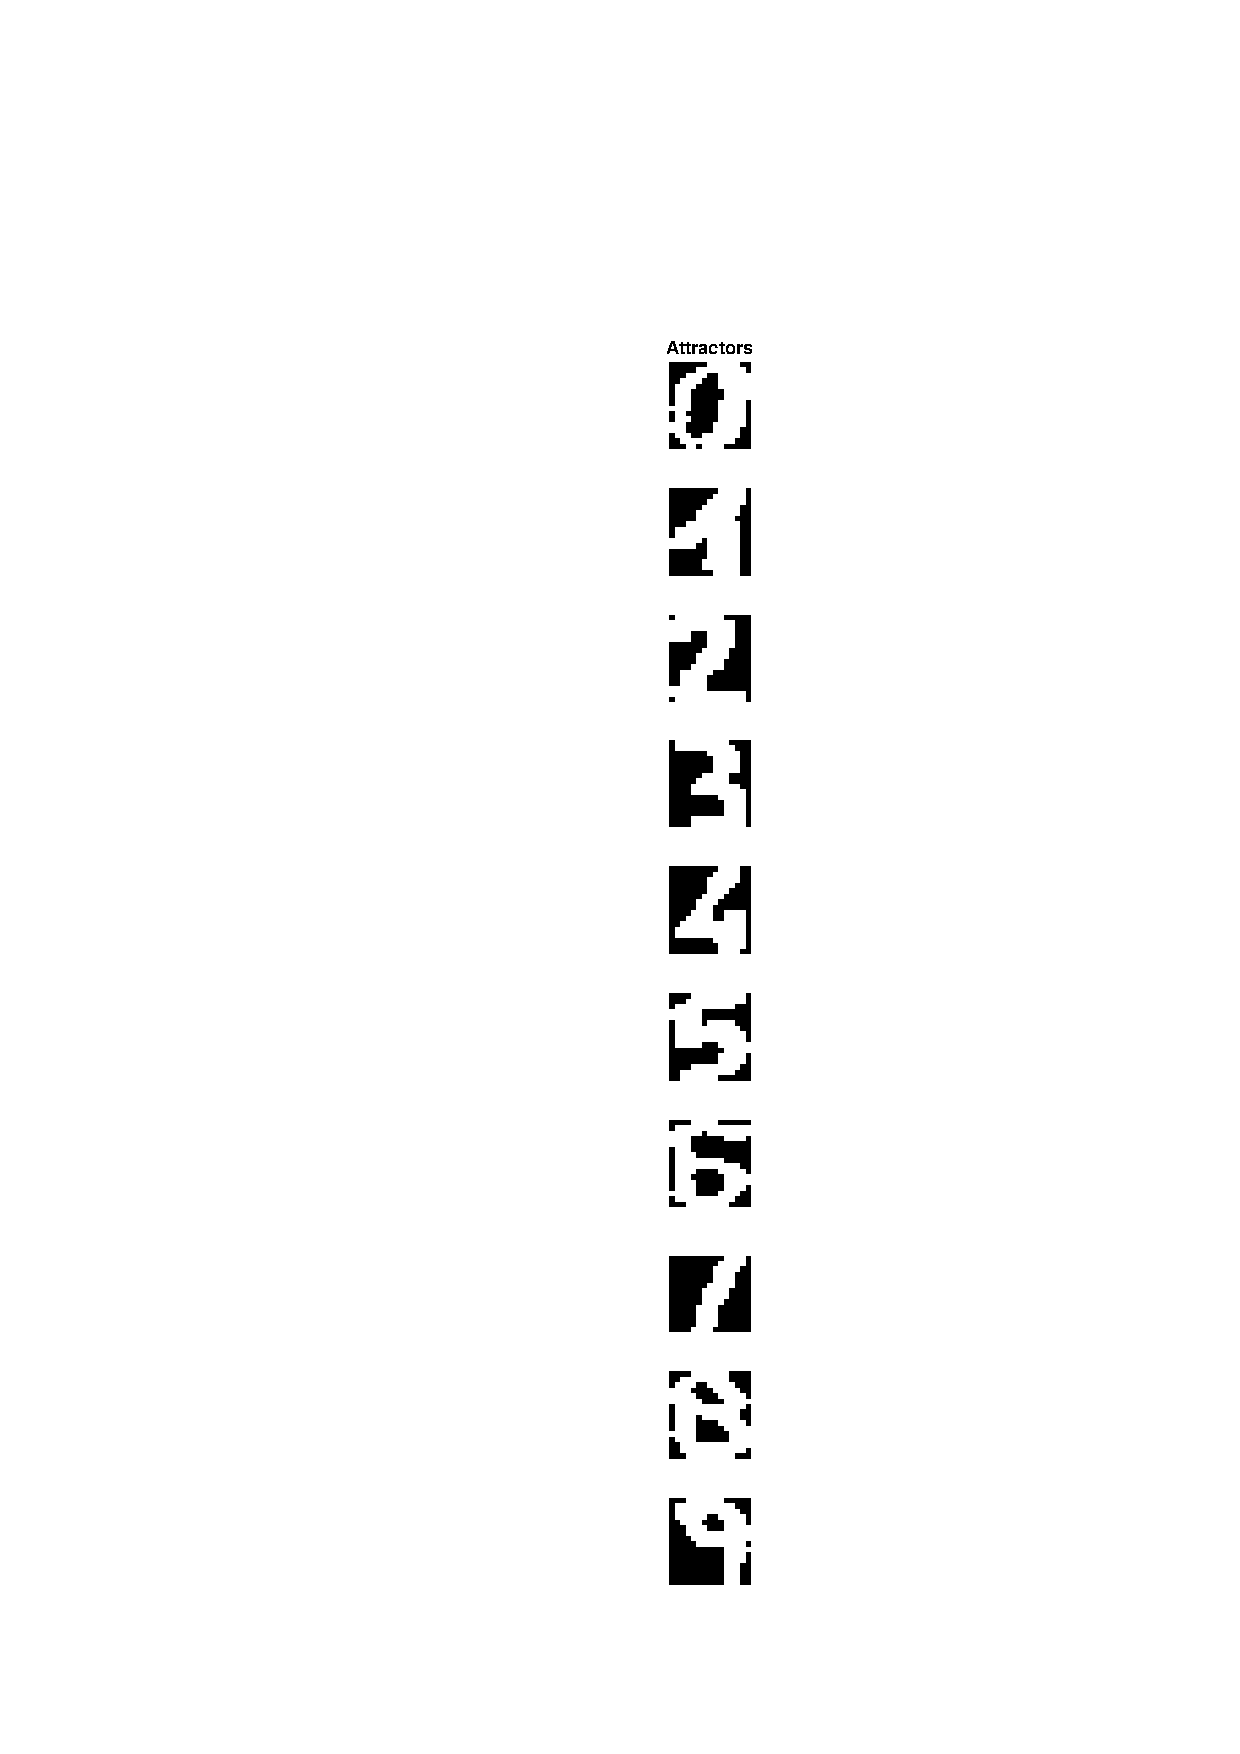
\includegraphics[height = 1.2\textwidth,width = 0.8\textwidth]{Exercise2/Report/hdr_n10_itr50.jpg}
		\caption{Noise Level = 10; Iterations = 50}\label{fig:hop_digit3}
	\end{subfigure}%
	\begin{subfigure}[b]{0.26\textwidth}
		\centering
		\captionsetup{width=0.8\linewidth, format = hang}
		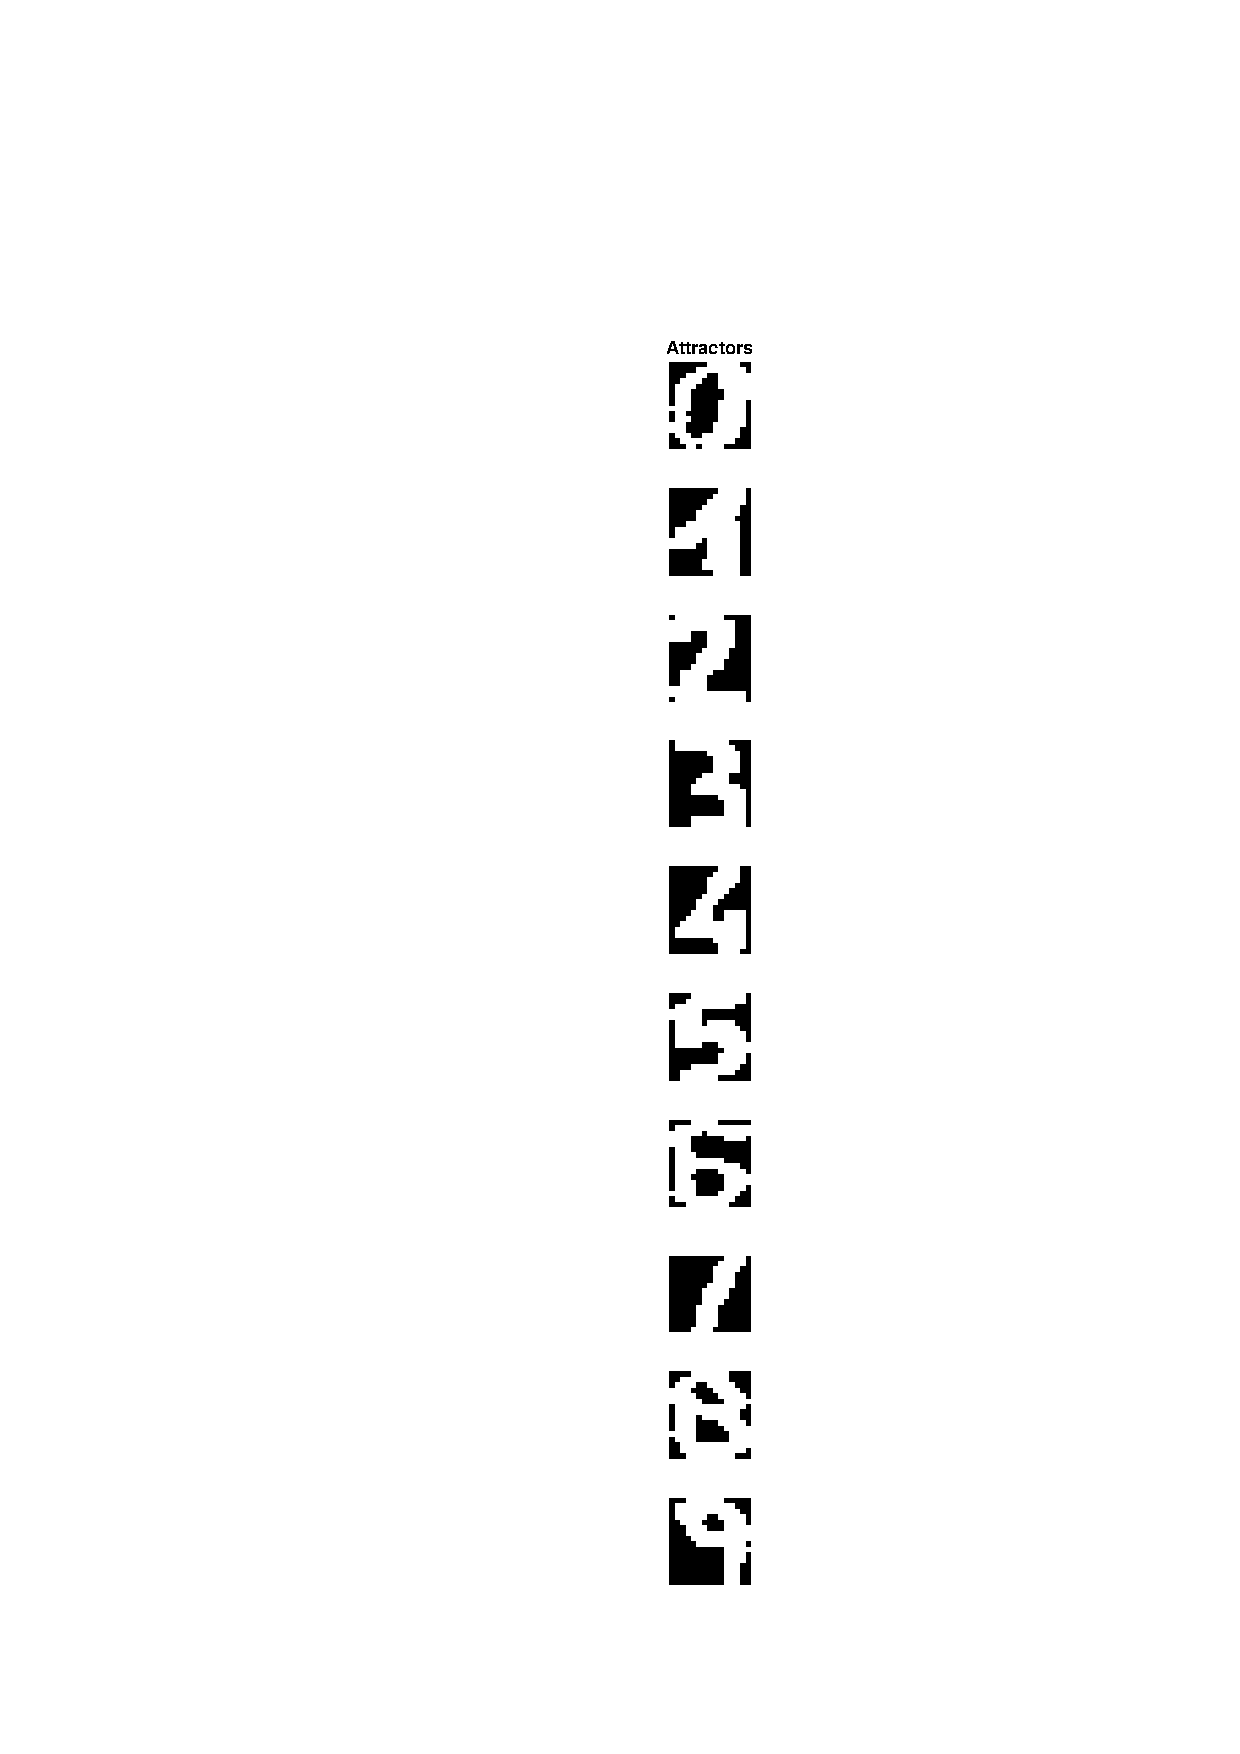
\includegraphics[height = 1.2\textwidth,width = 0.8\textwidth]{Exercise2/Report/hdr_n10_itr100.jpg}
		\caption{Noise Level = 10; Iterations = 100}\label{fig:hop_digit4)}
	\end{subfigure}%
	\caption{Hopfield Network for handwritten digit recognition}
	\label{fig:hop_digit}
\end{figure}\\
\section{Long Short-Term Memory Networks}
In this session we will train a recurrent multi-layer perceptron (MLP) and a LSTM network on Santafe dataset. The MLP network has limited capability of predicting a sample for only one step in the future. For this purpose, we iterate the network prediction for every step to predict one step into the future. We train this network using feed-forward with back propagation. On the other hand, LSTM networks are built to overcome the issue of long term dependencies which a normal recurrent neural network fails to learn. The LSTM network is made of a special memory cells which consists of gates. These gates learn and control the information flow in the network. They decide on if an information is to be passed on to further nodes or to be thrown away. Therefore, during training the network learn three different weight matrices namely $W_i$ corresponding to input gate, $W_f$ for forget gate and $W_o$ for output gate. The three gates can be characterized by the following equations Input Gate; $I(t) = \sigma (W_i x(t) + U_i h(t−1) + b_i)$, Forget Gate; $F(t) = \sigma (W_f x(t) + U_f h(t−1) + b_f)$ and Output Gate; $O(t) = \sigma (W_o x(t) + U_o h(t−1)+b_o)$, where $h(t-1)$ is a hidden state at time $t-1$ and $x(t)$ is the input at time $t$. 
\subsection{Time-series Prediction and Long short-term memory network}
Time series prediction using a MLP is explored with on hidden layers and various hidden units. The model is trained with different lags on the data sets to evaluate its performance because lags can change the number of training samples and training features. Therefore, the model is evaluated for lags in the range of 10 to 90 and (50; 100; 200) for the number of hidden units in a layer. The network is trained for 500 epochs for each of these hyper parameters and their corresponding RSME values are shown in the below figures. From figure \ref{fig:mlp_forecast}, it can be seen that for the first part of the test set where there are smaller spikes, the model performs better and gives a good prediction. But in the second part where there are huge spikes, the recurrent MLP failes to give a good prediction. The figure shown here is with a network having 100 hidden units in a layer. The overall performance of this network is not that great as it has an RMSE of 56.32 (\%). One major disadvantage of recurrent neural networks is that they suffer from vanishing gradients during back propagation. This can be over come by using LSTM's.

As seen from figures \ref{fig:lstm_forecast} and \ref{fig:lstm_updates}, the LSTM network predicts better than the MLP network on the test set. The RMSE values of LSTM network without the updates is 30.5863 which is still a higher value but smaller compared to the MLP network. When updates are taken into consideration, the RMSE value further reduces to 4.7167 which indicates that LSTM out performs the ordinary recurrent neural network.
\begin{figure}[!htpb] 
	\centering
	\begin{subfigure}[b]{0.33\textwidth}
		\captionsetup{width=0.8\linewidth, format = hang}
		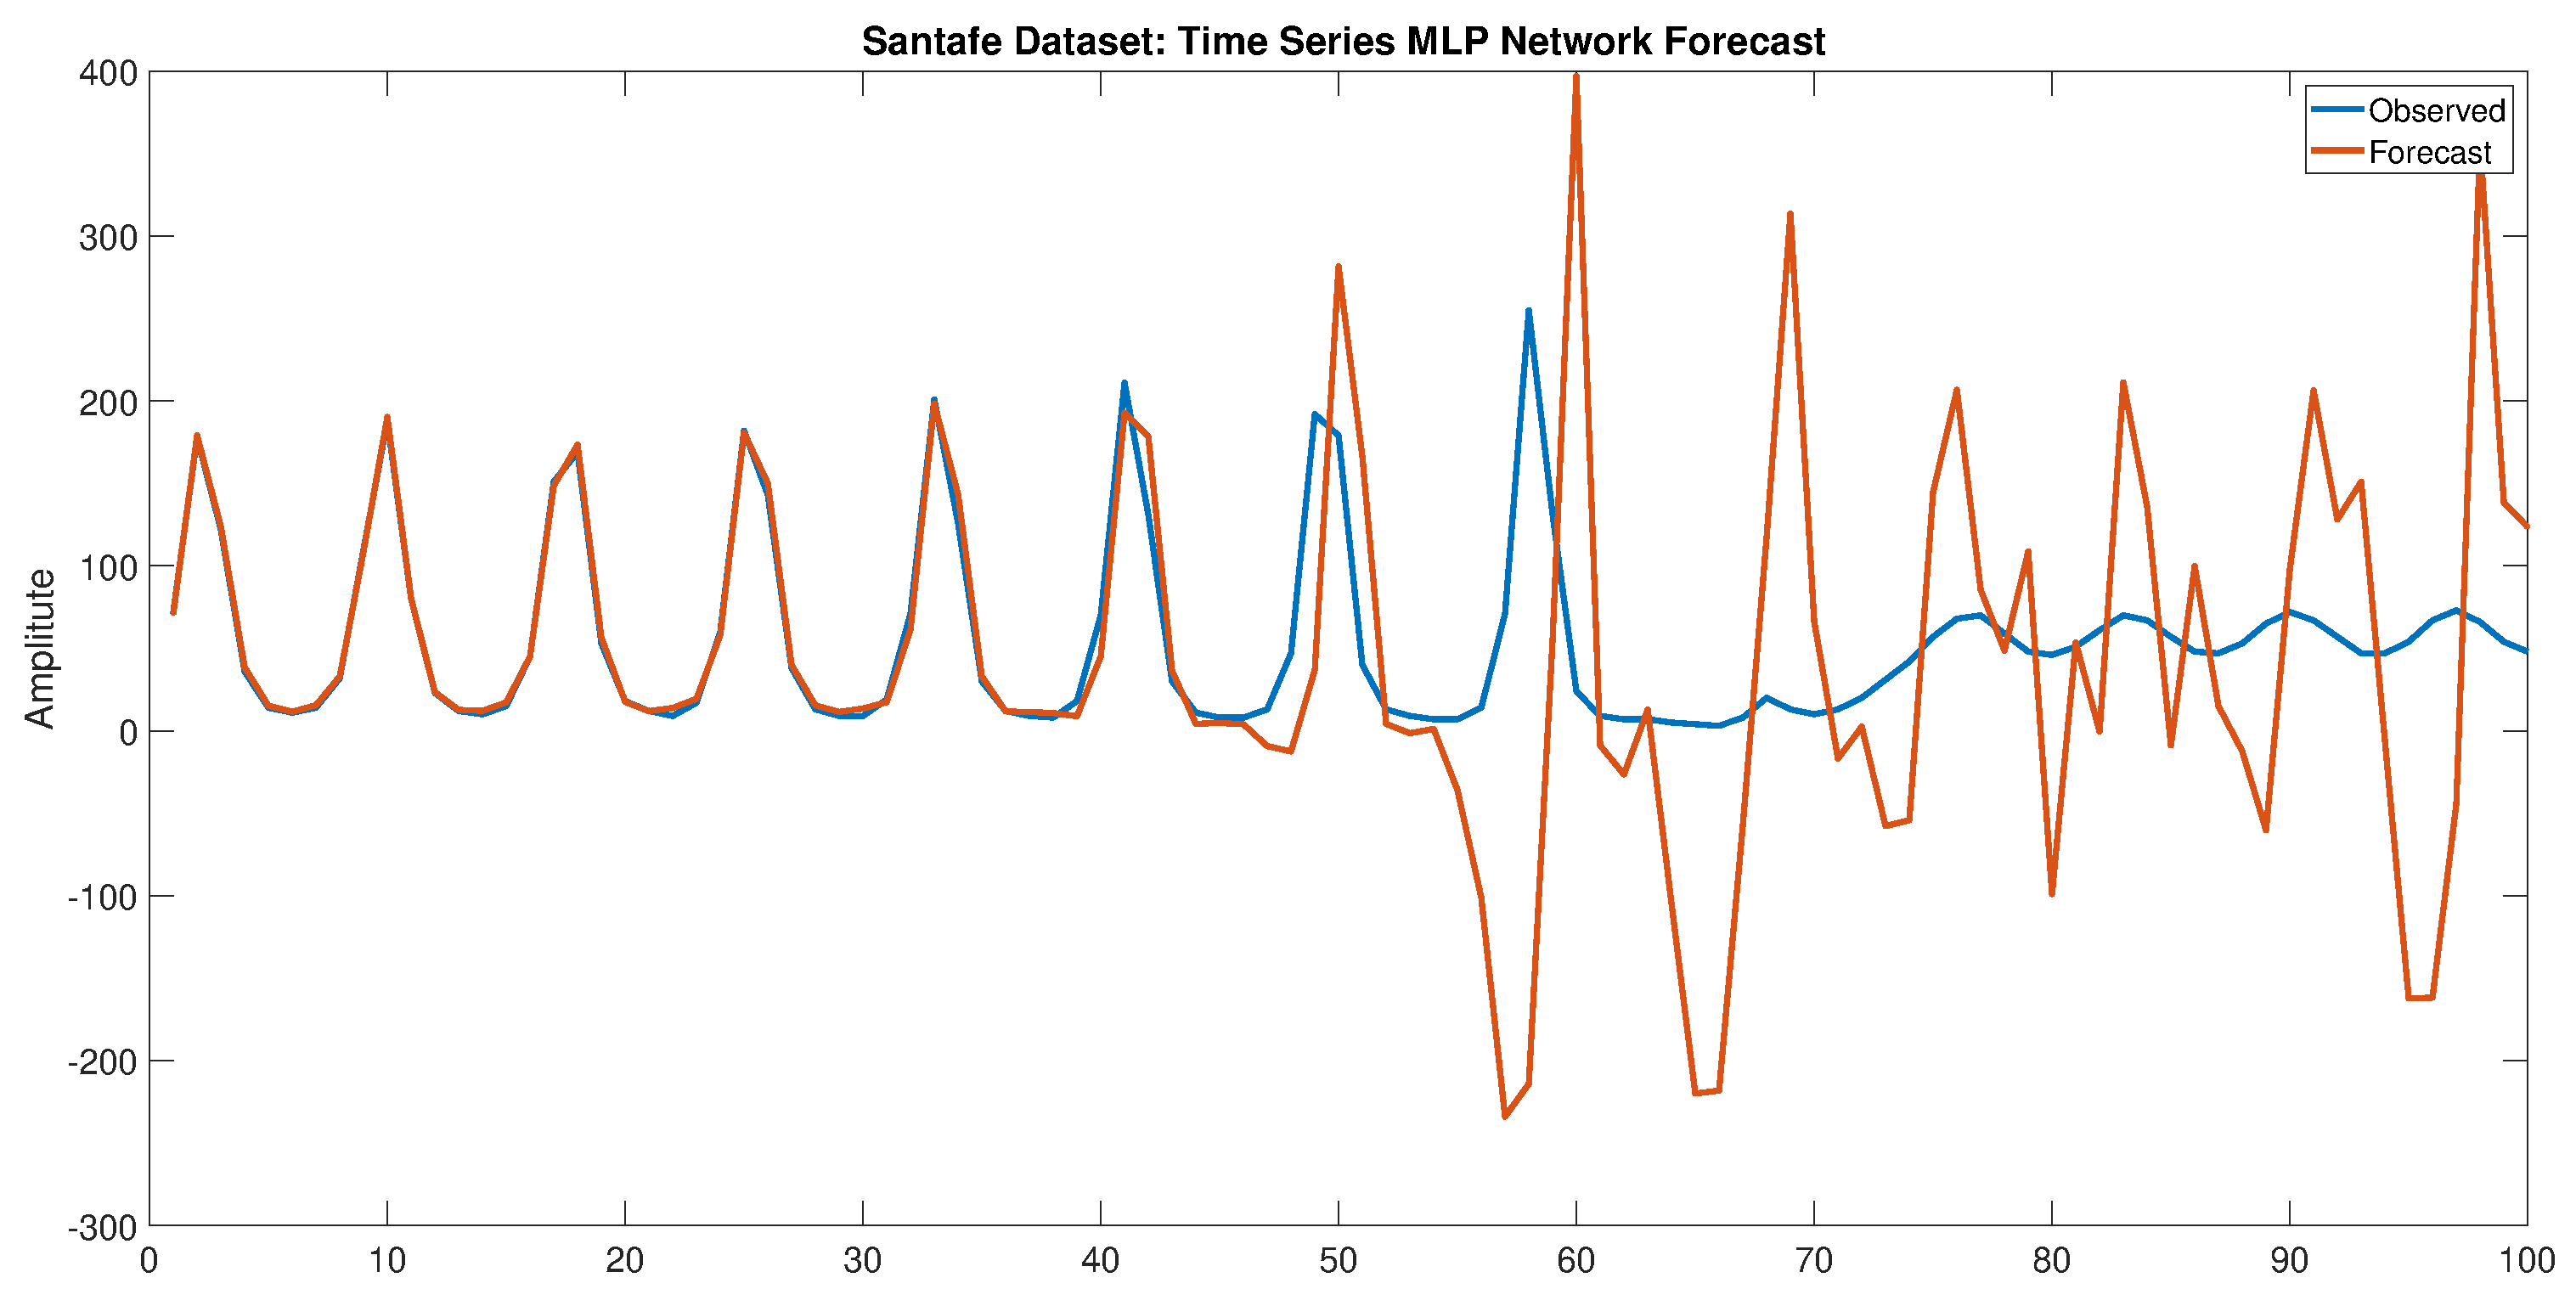
\includegraphics[height = 0.8\textwidth,width = 1\textwidth]{Exercise2/Report/mlp_forecast}
		\caption{MLP Network; Actual and Predicted output on test data }\label{fig:mlp_forecast}
	\end{subfigure}%
	\begin{subfigure}[b]{0.33\textwidth}
		\captionsetup{width=0.8\linewidth, format = hang}
		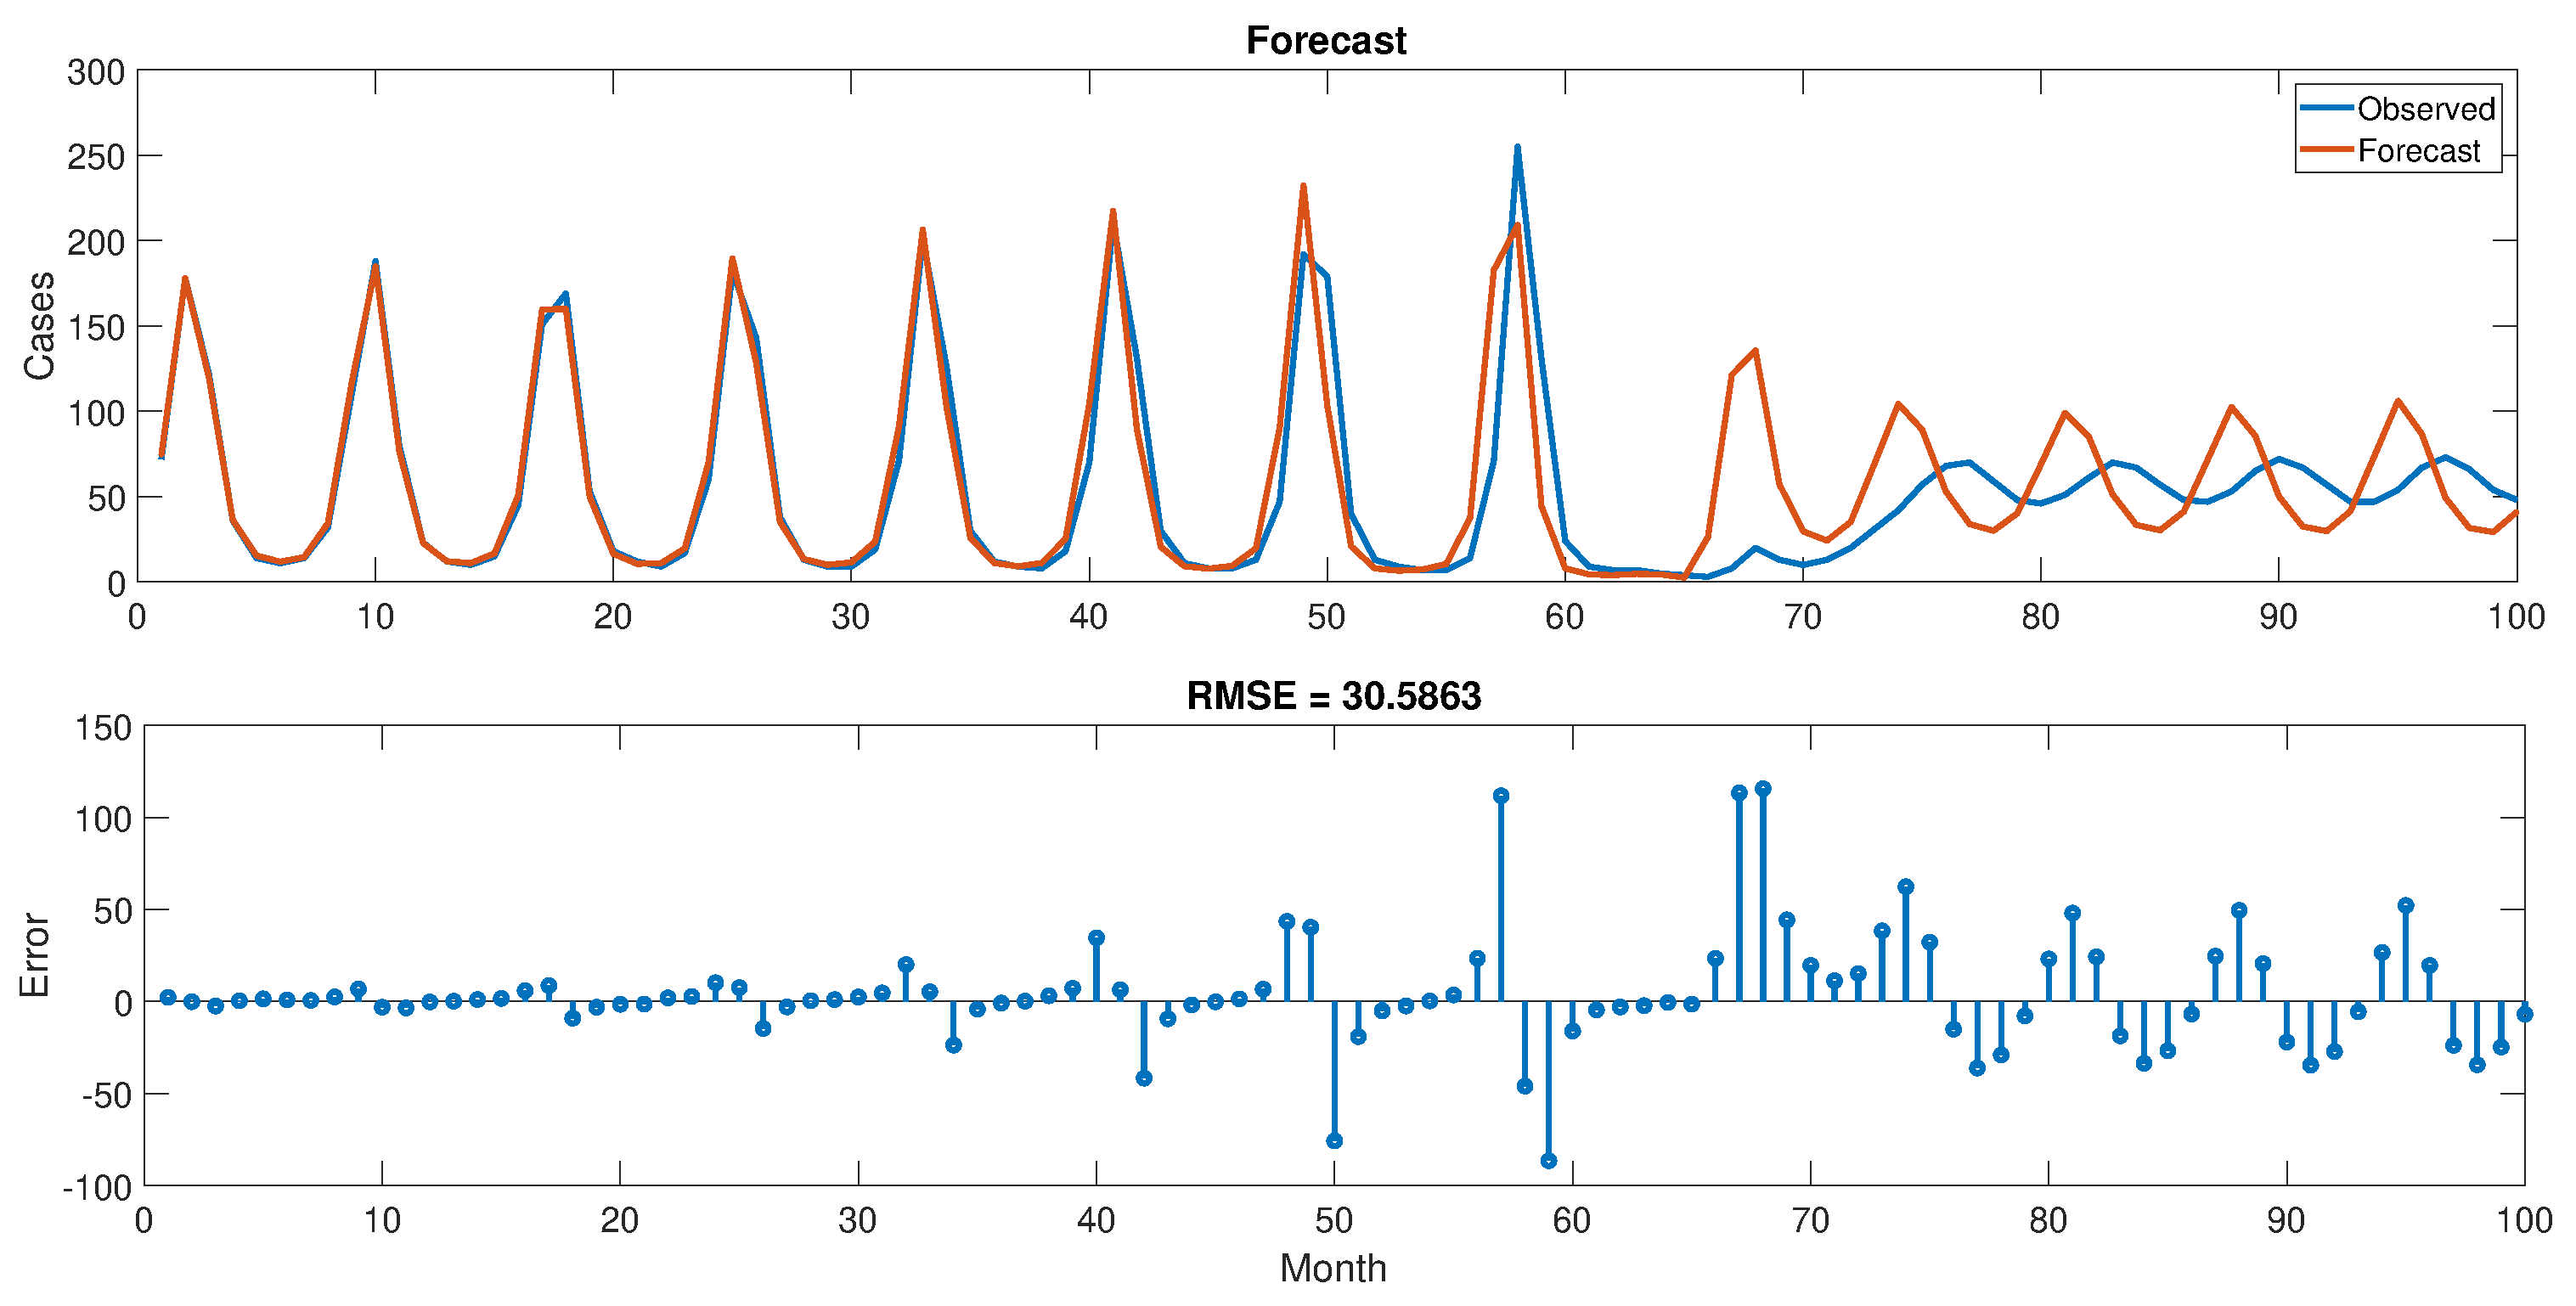
\includegraphics[height = 0.8\textwidth,width = 1\textwidth]{Exercise2/Report/lstm_forecast}
		\caption{LSTM Network; Actual and Predicted output on test data}\label{fig:lstm_forecast}
	\end{subfigure}%
	\begin{subfigure}[b]{0.33\textwidth}
		\captionsetup{width=1\linewidth, format = hang}
		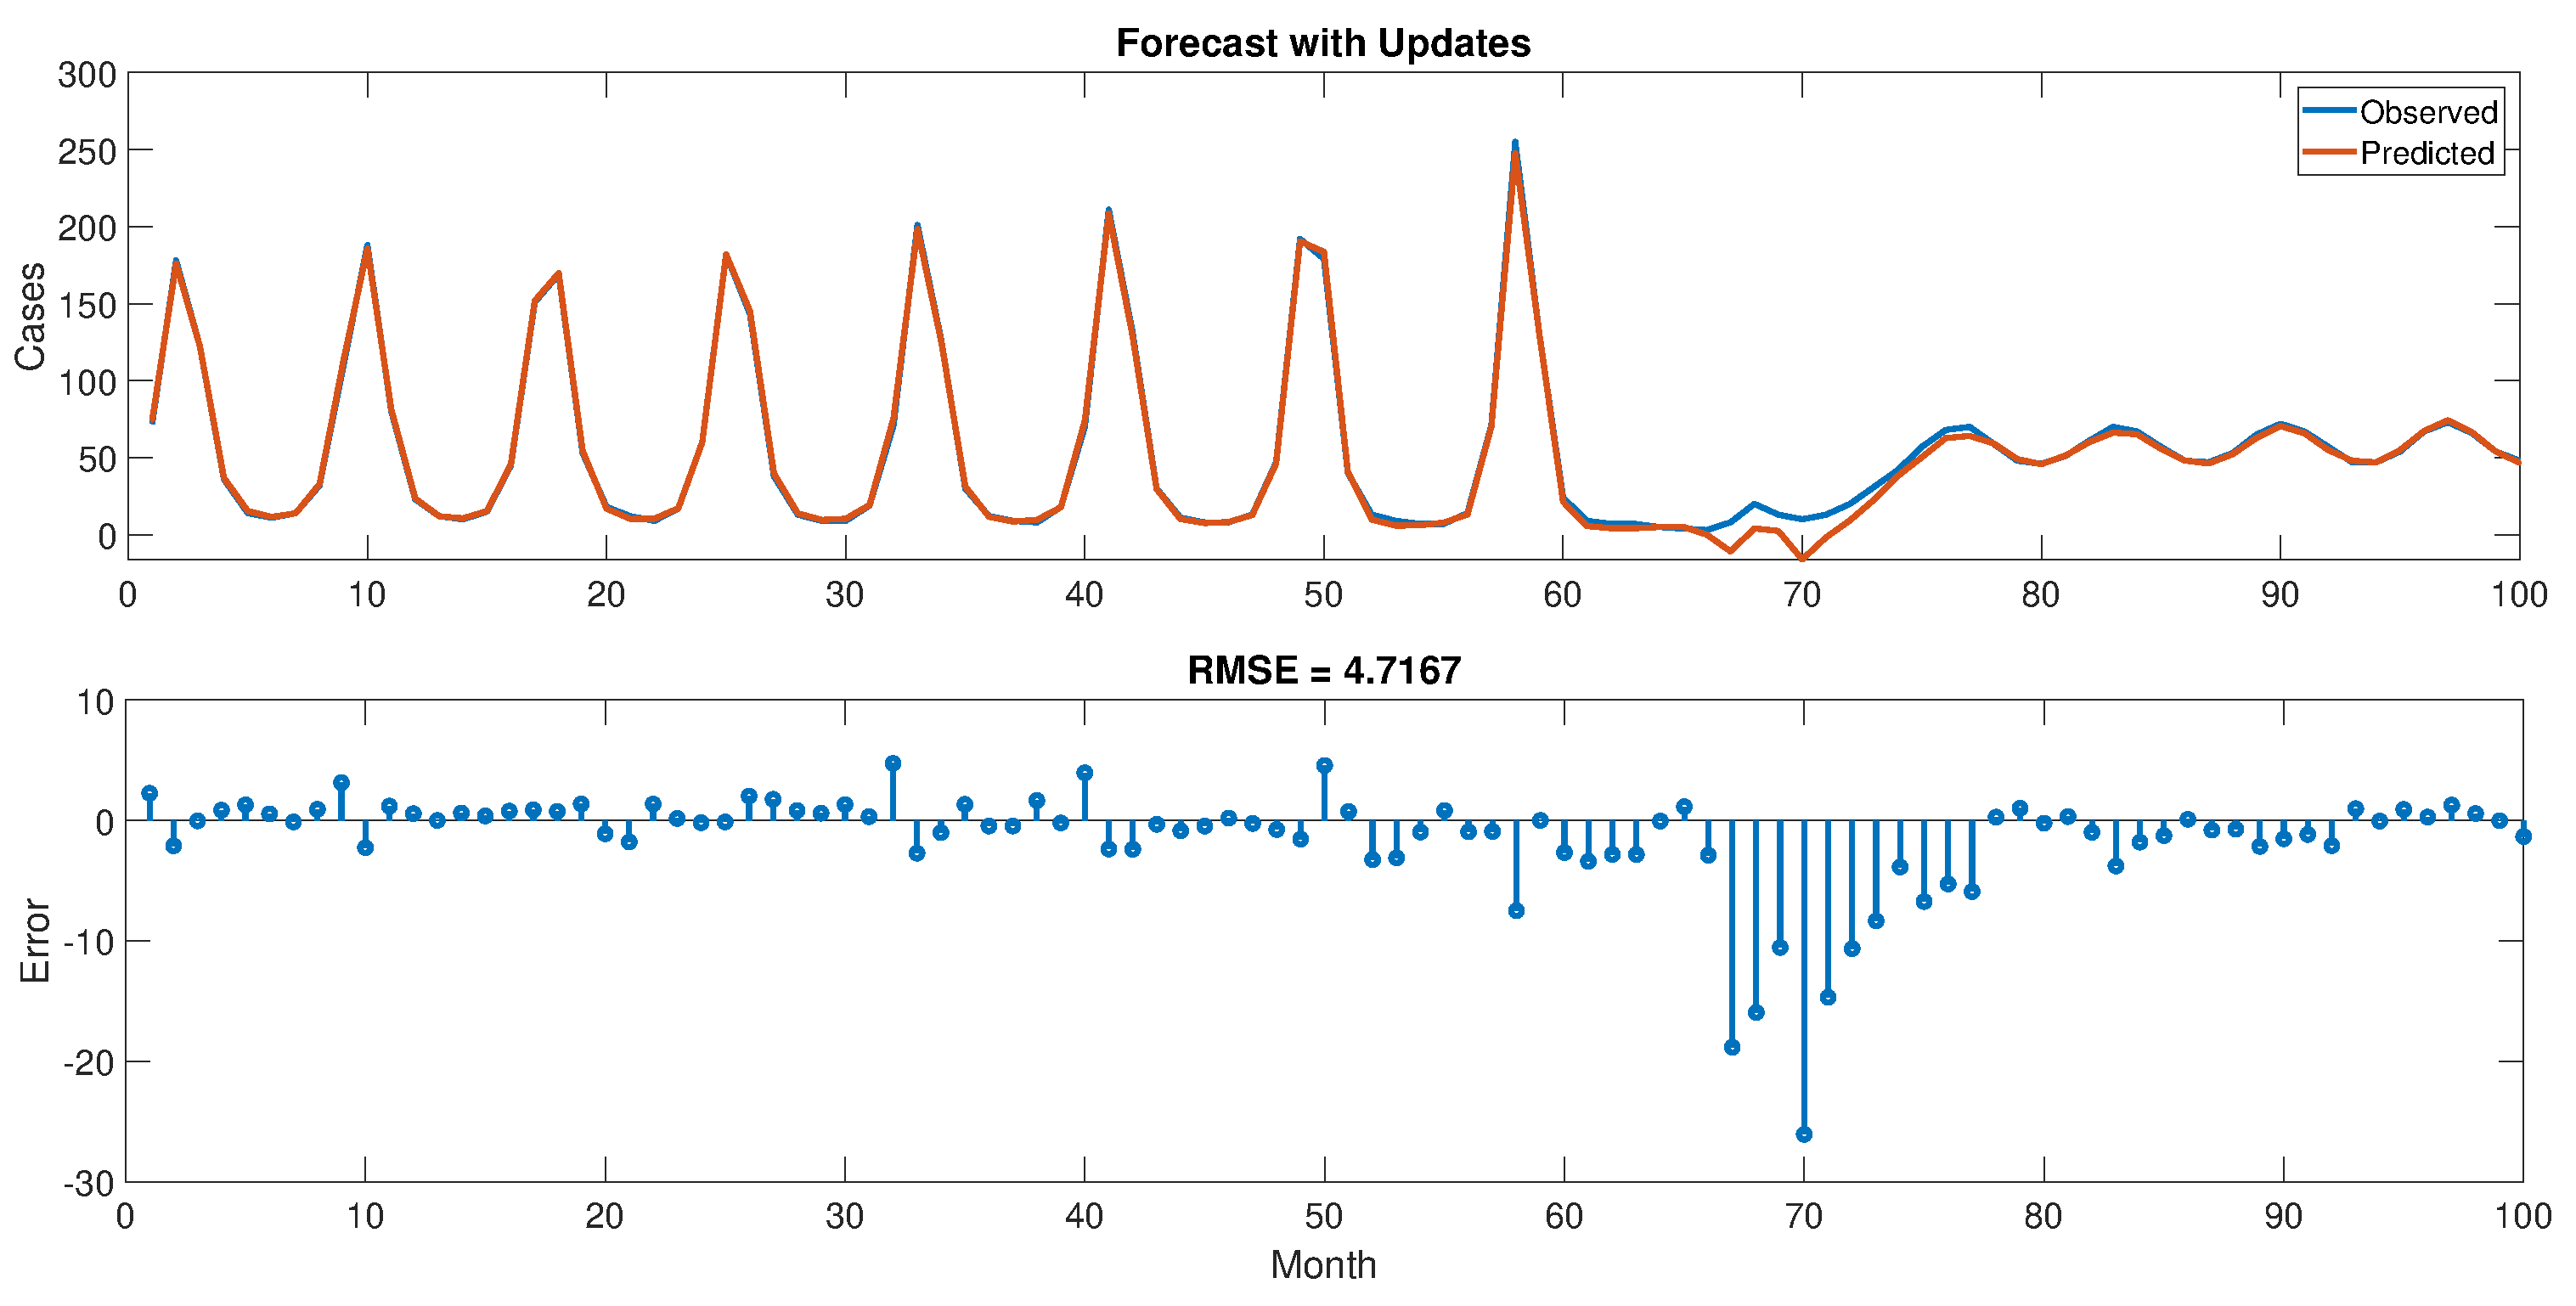
\includegraphics[height = 0.8\textwidth,width = 1\textwidth]{Exercise2/Report/lstm_forecast_update}	
		\caption{LSTM Network; Actual and Predicted output with updates on test data}\label{fig:lstm_updates}
	\end{subfigure}%
	\caption{Santafe Dataset; Actual and predicted outputs on test data with RMSE for MLP and LSTM networks}
	\label{fig:forecasts}
\end{figure}\\
The figure \ref{fig:lags} shows the performances of both the networks in case of change in lags and number of hidden units. It can be seen that the RMSE values over the number of lags for LSTM network is almost 10x times smaller compared to the recurrent MLP network. Therefore, using a LSTM network would be a better choice for all the above said reasons.
\begin{figure}[!htpb]
	\centering
	\begin{subfigure}[b]{0.45\textwidth}
		\captionsetup{width=0.8\linewidth, format = hang}
		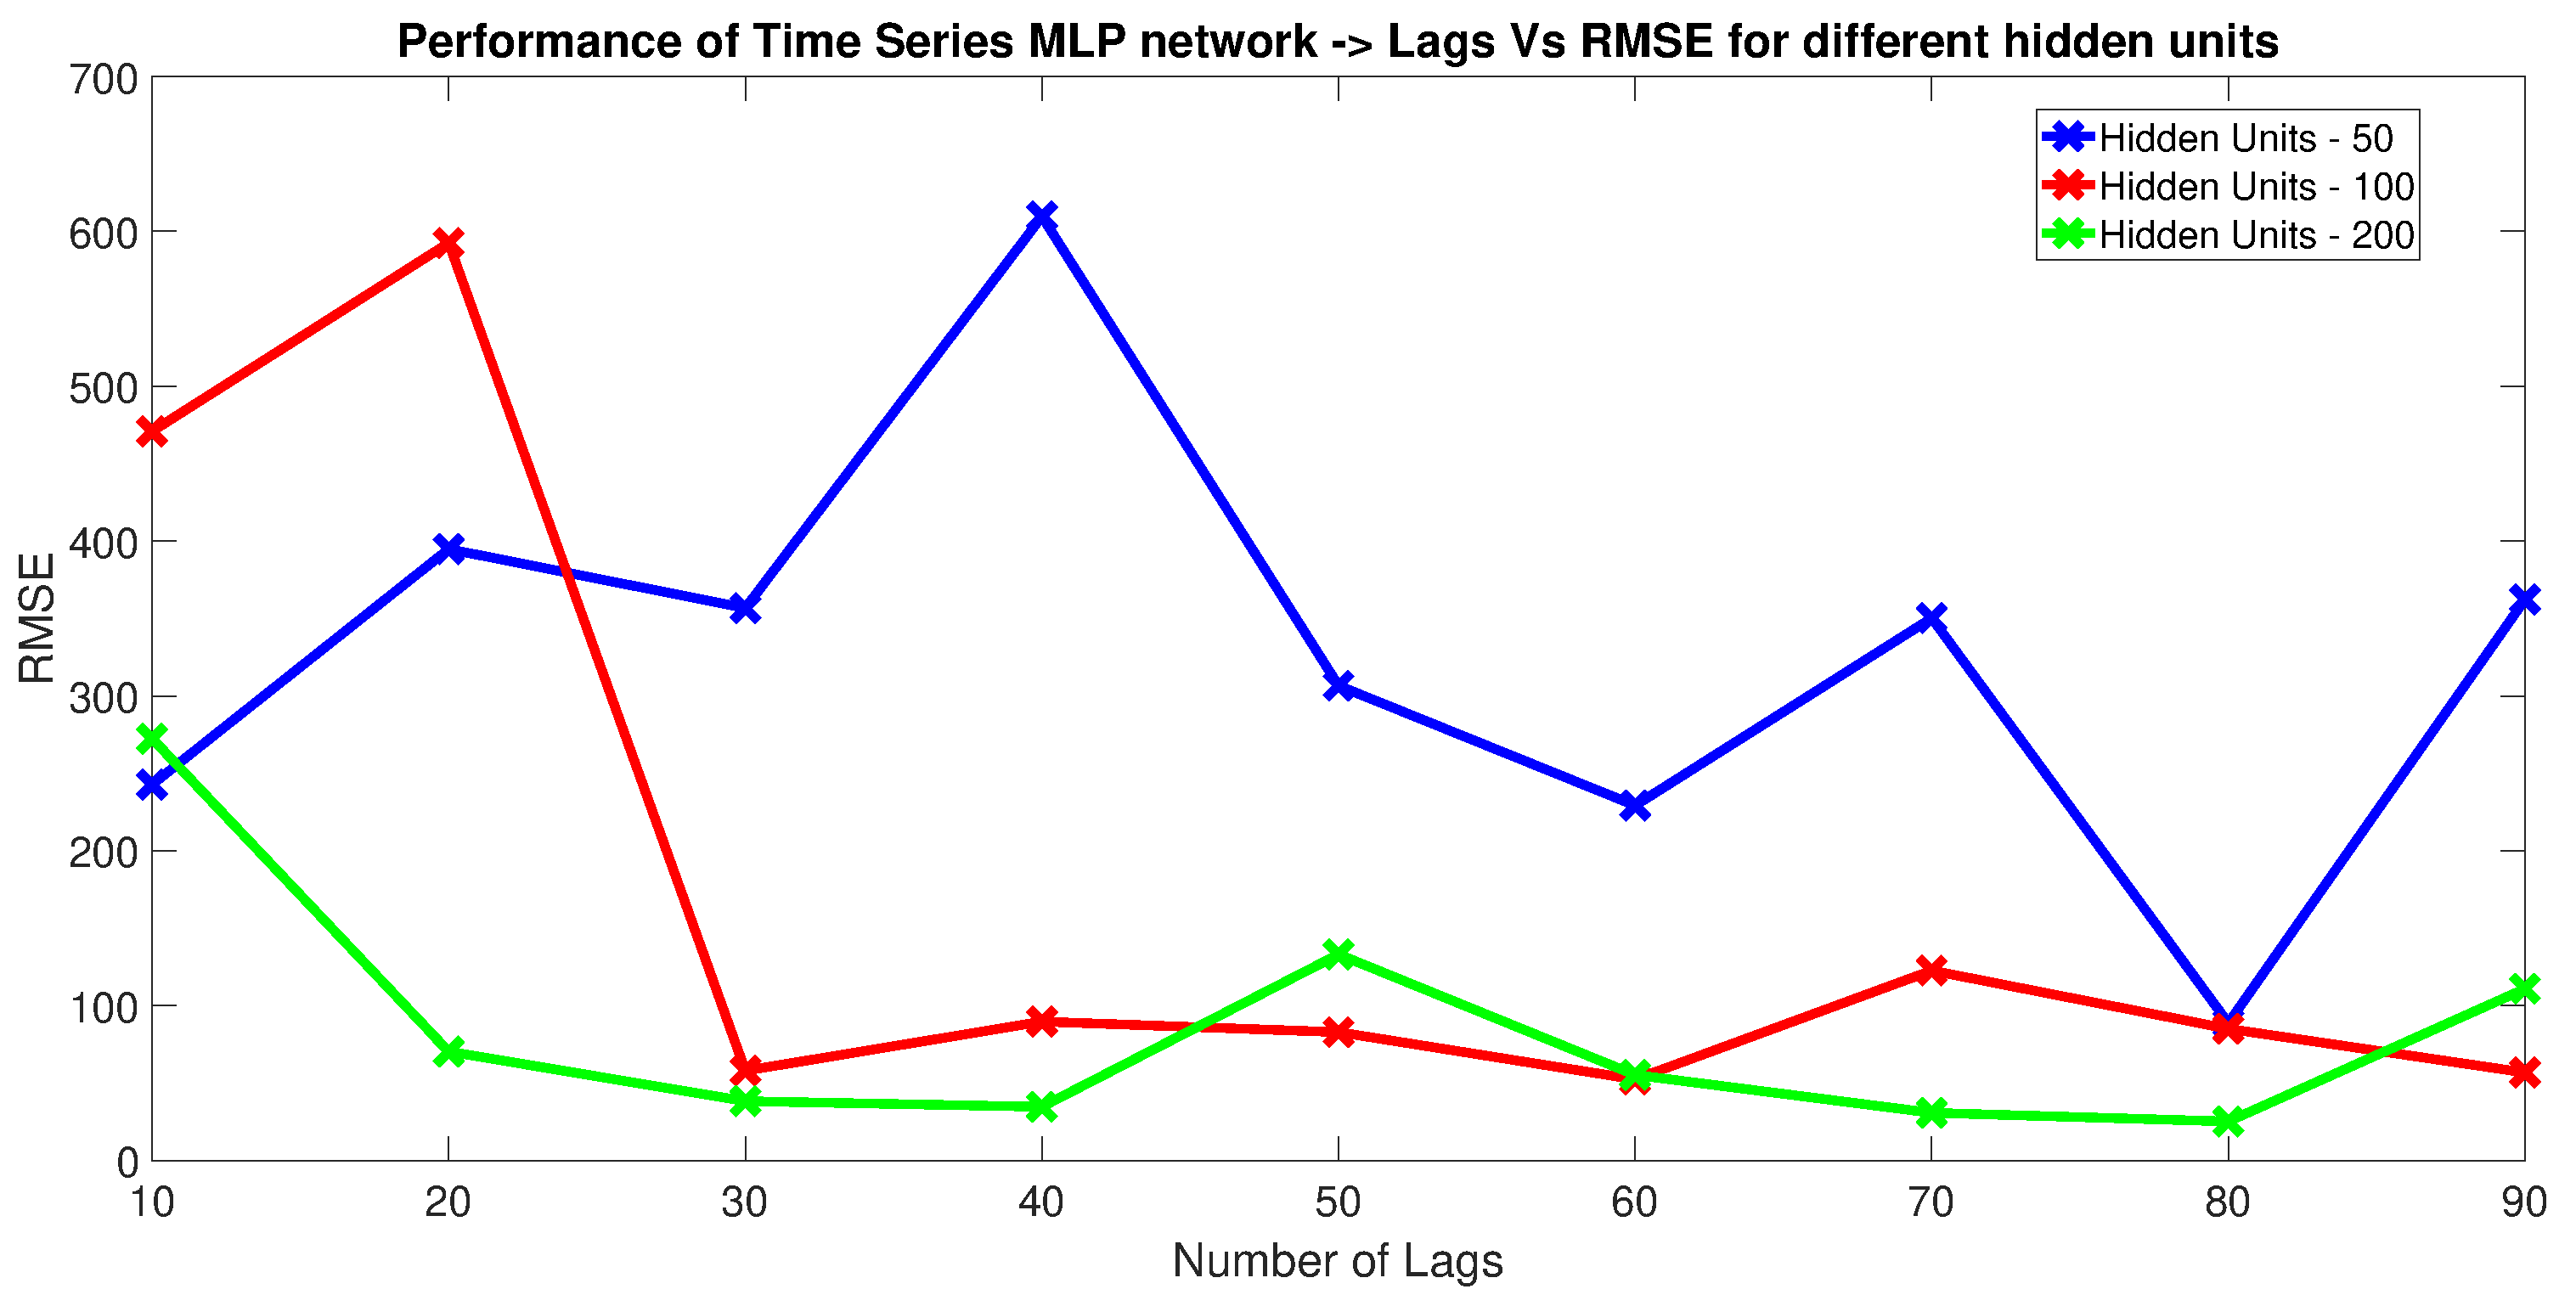
\includegraphics[height = 0.52\textwidth,width = 1\textwidth]{Exercise2/Report/mlp_lags}
		\caption{MLP Network; Number of Lags Vs RMSE for (50, 100, 200) hidden units }\label{fig:mlp_lags}
	\end{subfigure}%
	\begin{subfigure}[b]{0.45\textwidth}
		\captionsetup{width=0.8\linewidth, format = hang}
		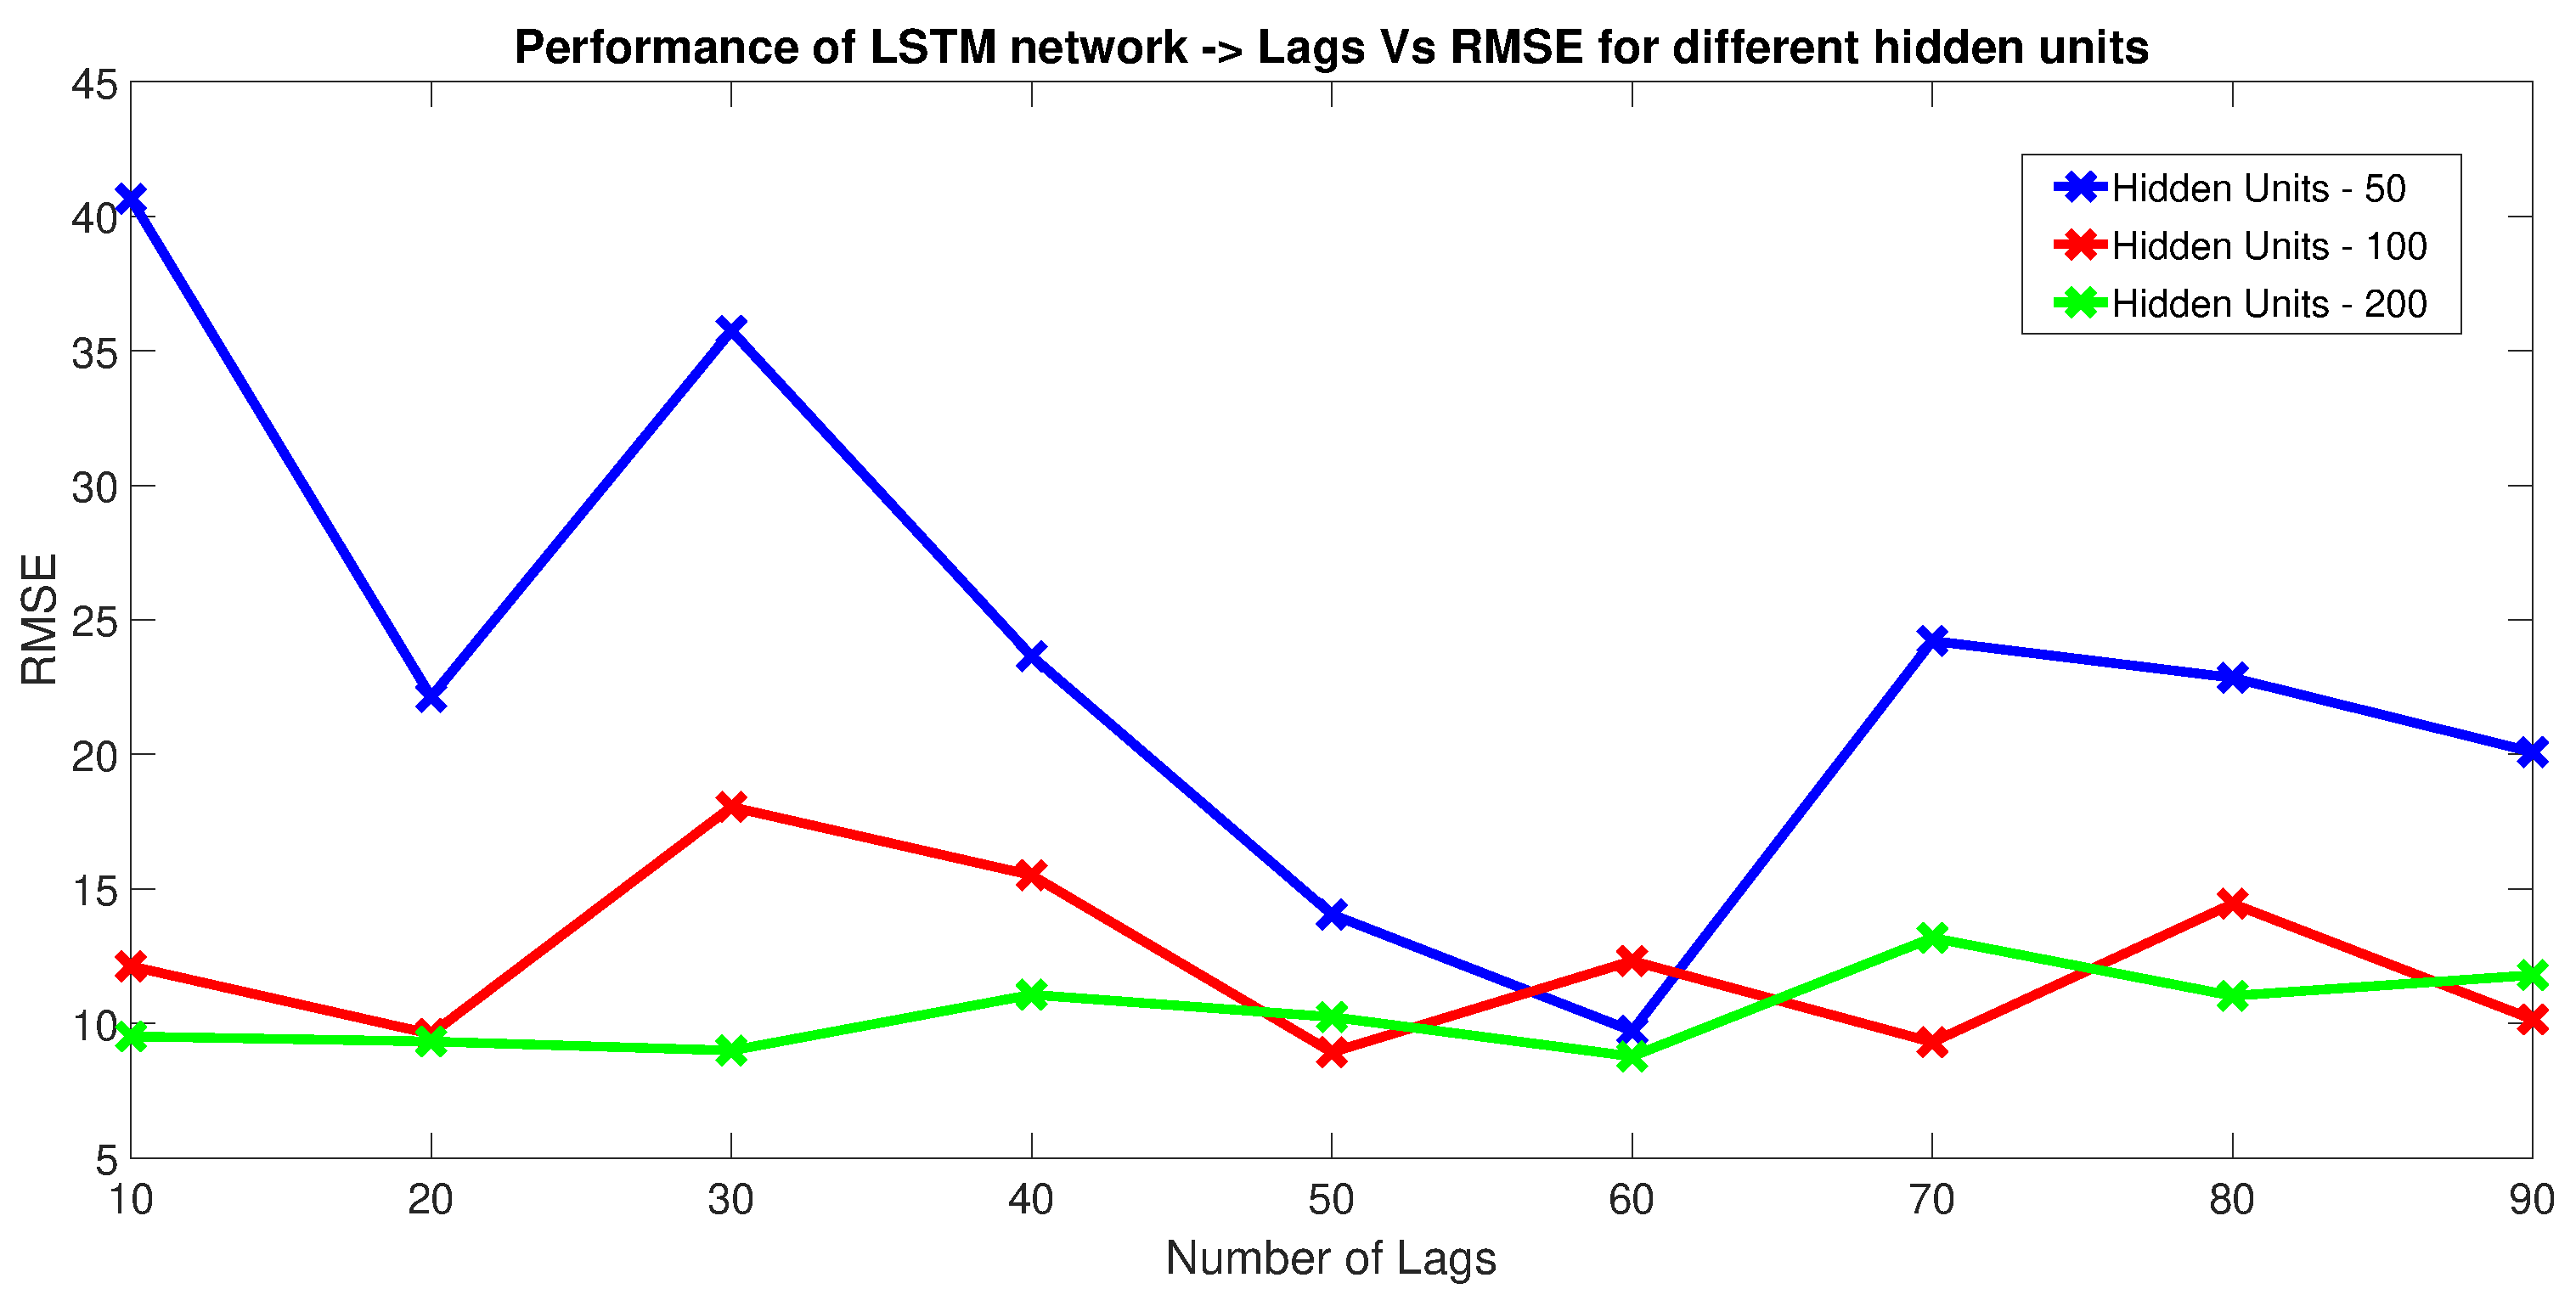
\includegraphics[height = 0.52\textwidth,width = 1\textwidth]{Exercise2/Report/lstm_lags}
		\caption{LSTM Network; Number of Lags Vs RMSE for (50, 100, 200) hidden units }\label{fig:lstm_lags}
	\end{subfigure}%
	\caption{Santafe Dataset; Number of Lags Vs RMSE for MLP and LSTM networks}
	\label{fig:lags}
\end{figure}